\documentclass[xcolor=dvipsnames, compress, 12pt, aspectratio=169, handout]{beamer}
\usetheme{Boadilla}
\useinnertheme{circles} % make bullets matte
\setbeamertemplate{footline}[frame number]
\setbeamertemplate{section in toc}[sections numbered]
\setbeamertemplate{subsection in toc}[sections numbered]
\setbeamertemplate{navigation symbols}{} 
\setbeamercovered{transparent}
\usepackage{graphicx}
\usepackage{hhline}
\usepackage{appendixnumberbeamer}
\definecolor{maincolor}{rgb}{0.6, 0.4, 0.7}
\usecolortheme[named = maincolor]{structure}
\renewcommand{\arraystretch}{1.5}
\usepackage{bbm}

\title{Who Pays the Cost of Exclusion?: Selection into Immigration Under the 1885 Chinese Head Tax}
\author{Amy Kim}
\institute{Princeton University}
\date{January 18, 2024}

\begin{document}
\begin{frame}[plain]
    \titlepage
\end{frame}

%%%%%%%%%%%%%%%%%%%%%%%%%%%
%%%% INTRODUCTION
%%%%%%%%%%%%%%%%%%%%%%%%%%%
\section{Introduction}
\begin{frame}
    \frametitle{Introduction}
    \begin{itemize}
        \item Complex immigration system in U.S. and Canada $\implies$ variety of \textbf{costs} 
        \vspace{1mm}
        \begin{itemize}
            \item $\sim$31k CAD for family of 4 to immigrate to Canada \textcolor{gray}{RBC 2023}
        \end{itemize}
        \vspace{2mm}
        \item Potential implications for (1) immigration flows \& (2) immigrant characteristics
        \vspace{2mm}
        \item But migration cost generally hard to measure and likely endogenous
        \vspace{2mm}
        \item \textbf{Exception:} 1885 Chinese Head Tax
        \begin{itemize}
            \vspace{1mm}
            \item Fixed per-person immigration fee only for Chinese immigrants to Canada
            \vspace{1mm}
            \item Exogenous variation in fee over time -- by 1903, \$500 ($\sim$19k CAD today)
            \vspace{1mm}
            \item Detailed data on fees and immigrant characteristics at arrival $+$ census 
        \end{itemize}
    \end{itemize}
\end{frame}

\begin{frame}
    \frametitle{This Paper}
    \textbf{How did the Chinese Head Tax affect Chinese immigration to Canada?}
    \vspace{2mm}
    \begin{enumerate}
        \item Direct effect of Head Tax on inflow of Chinese immigrants 
        \vspace{3mm}
        \begin{itemize}
            \item \textbf{Result:} 80\% $\downarrow$ in Chinese imm. at peak of Head Tax
        \end{itemize}
        \vspace{3mm}
        \item Effect of Head Tax on selection of Chinese immigrants into migration 
        \vspace{2mm}
        \begin{itemize}
            \item \textbf{Result:} Chinese immigrants more positively selected when Head Tax $\uparrow$
            \vspace{1mm}
            \begin{itemize}
                \item $\uparrow$ avg. height, literacy, home ownership \vspace{1mm}
                \item $\downarrow$ probability of being a laborer
            \end{itemize}
        \end{itemize}
    \end{enumerate}
\end{frame}

\begin{frame}
    \frametitle{Literature Review}
    \begin{itemize}
        \item Immigration Policy \small \textcolor{gray}{Clemens et al. 2018, Feigenberg 2020, Abramitzky et al. 2023}
        \vspace{2mm}
        \begin{itemize}
            \item Chinese immigration: using census only \footnotesize \textcolor{gray}{Chen 2015, Chen and Xie 2020}
            \vspace{1mm} \small 
            \item \textbf{My Contribution:} Detailed migration microdata + understudied imm. group 
        \end{itemize}
        \vspace{2mm} \normalsize 
        \vspace{2mm} 
        \item Selection into migration \small \textcolor{gray}{Roy 1951, Borjas 1987}
        \vspace{2mm}
        \begin{itemize}
            \item Historical: no cost \footnotesize \textcolor{gray}{Abramitzky et al. 2013, Abramitzky and Boustan 2017, Connor 2019} \vspace{1mm}
            \item \small Modern: high `cost' but hard to measure \footnotesize \textcolor{gray}{McKenzie and Rapoport 2010, Ortega and Peri 2013, Angelucci 2015, Cai 2020, Feigenberg 2020} \vspace{1mm} 
            \item \small \textbf{My Contribution:} historical setting + high cost 
        \end{itemize} \normalsize 
    \end{itemize}
\end{frame}

%%% TABLE OF CONTENTS
\begin{frame}[plain]{Outline}
    \tableofcontents
    \addtocounter{framenumber}{-1}
\end{frame}

%%% TABLE OF CONTENTS -- CURRENT SECTION
\AtBeginSection[ ]
{
\begin{frame}[plain]{Outline}
    \tableofcontents[currentsection, hideothersubsections]
    \addtocounter{framenumber}{-1}
\end{frame}
}


%%%%%%%%%%%%%%%%%%%%%%%%%%%
%%%% HISTORICAL BACKGROUND
%%%%%%%%%%%%%%%%%%%%%%%%%%%
\section{Historical Context}
\begin{frame}
    \frametitle{Chinese Immigration to Canada}
    \begin{columns}
        \begin{column}{0.5\textwidth}
            \begin{figure}
                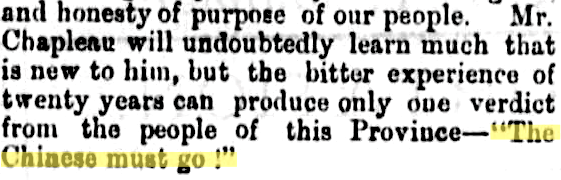
\includegraphics[width=\textwidth]{../../figs/slides/portmoody_1884.png}
                \caption{\textcolor{gray}{Port Moody Gazette, August 23 1884}}
            \end{figure}
            \begin{figure}
                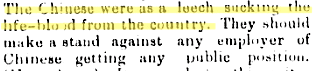
\includegraphics[width=\textwidth]{../../figs/slides/victoria_1885.png}
                \caption{\textcolor{gray}{Victoria Daily Colonist, June 16 1885}}
            \end{figure}
        \end{column}
        \begin{column}{0.5\textwidth}  
            \begin{itemize}
                \item 1850s and 1860s: West Coast Gold Rush
                \vspace{2mm}
                \item 1880s: Canadian Pacific Railway
                \vspace{2mm}
                \item 1882: U.S. Chinese Exclusion Act
                \vspace{2mm}
                \item July 1885: Canada's Chinese Immigration Act
            \end{itemize}
        \end{column}
    \end{columns}
\end{frame}

\begin{frame}
    \frametitle{Chinese Head Tax}
    \label{headtaxinfo}
    \begin{itemize}
        \item Initial 1885 Head Tax: \$50 ($\approx$ 2k CAD today)
        \begin{itemize}
            \vspace{1mm}
            \item Exceptions for diplomats, merchants, students (less than 9\% of Chinese imm.)
        \end{itemize}
        \vspace{2mm}
        \item 1900 amendment -- increase to \$100 ($\approx$ 4k CAD) \vspace{2mm}
        \item 1903 amendment -- increase to \$500 ($\approx$ 19k CAD) \vspace{2mm}
        \item 1923 Chinese Immigration Act banned Chinese immigration altogether
    \end{itemize}
    \vspace{2mm}
    \hyperlink{fig_headtax}{\beamergotobutton{HT Certificate}} \hyperlink{figa1_tax}{\beamergotobutton{Adherence to Tax}}
\end{frame}

%%%%%%%%%%%%%%%%%%%%%%%%%%%
%%%% DATA
%%%%%%%%%%%%%%%%%%%%%%%%%%%
\section{Data}
\begin{frame}
    \label{data}
    \frametitle{Summary of Data Sources}
    \begin{enumerate}
        \item Register of Chinese Immigrants to Canada (1885-1949) \textcolor{gray}{Ward and Yu 2008} 
        \vspace{2mm}
        \begin{itemize}
            \item Record of all Chinese immigrants to Canada at time of entry \hyperlink{fig_register}{\beamergotobutton{Image}}
            \vspace{1mm}
            \item Full name, age, sex, occupation, height, tax paid, date \& port \& method of entry
            \vspace{1mm}
            \item Registration mandatory only for post-1885 arrivals, so no pre-period (\$0 tax)
        \end{itemize}
        \vspace{2mm}
        \item Hong Kong Harbourmaster Reports (1870-1930)
        \begin{itemize}
            \item Total immigrants (emigrants) from (to) HK by destination (origin) port \hyperlink{figa2_imm}{\beamergotobutton{CA imm/em}}
            \vspace{1mm}
            \item \textbf{This paper:} total immigration out of Hong Kong as `push factor' proxy
        \end{itemize}
        \vspace{2mm}
        \item Decennial Canadian Census (1881-1921) 
        \vspace{2mm}
        \begin{itemize}
            \item Includes year of immigration (starting in 1901) and birthplace 
            \vspace{1mm}
            \item Rich set of variables, but suffers from return migration attrition and measurement error
        \end{itemize}
    \end{enumerate}
\end{frame}

%%%%%%%%%%%%%%%%%%%%%%%%%%%
%%%% Direct Effects
%%%%%%%%%%%%%%%%%%%%%%%%%%%
\section{Effects on Immigration Inflow}
\begin{frame}
    \frametitle{$\downarrow$ in Chinese immigration when Head Tax $\uparrow$}
    \begin{figure}
        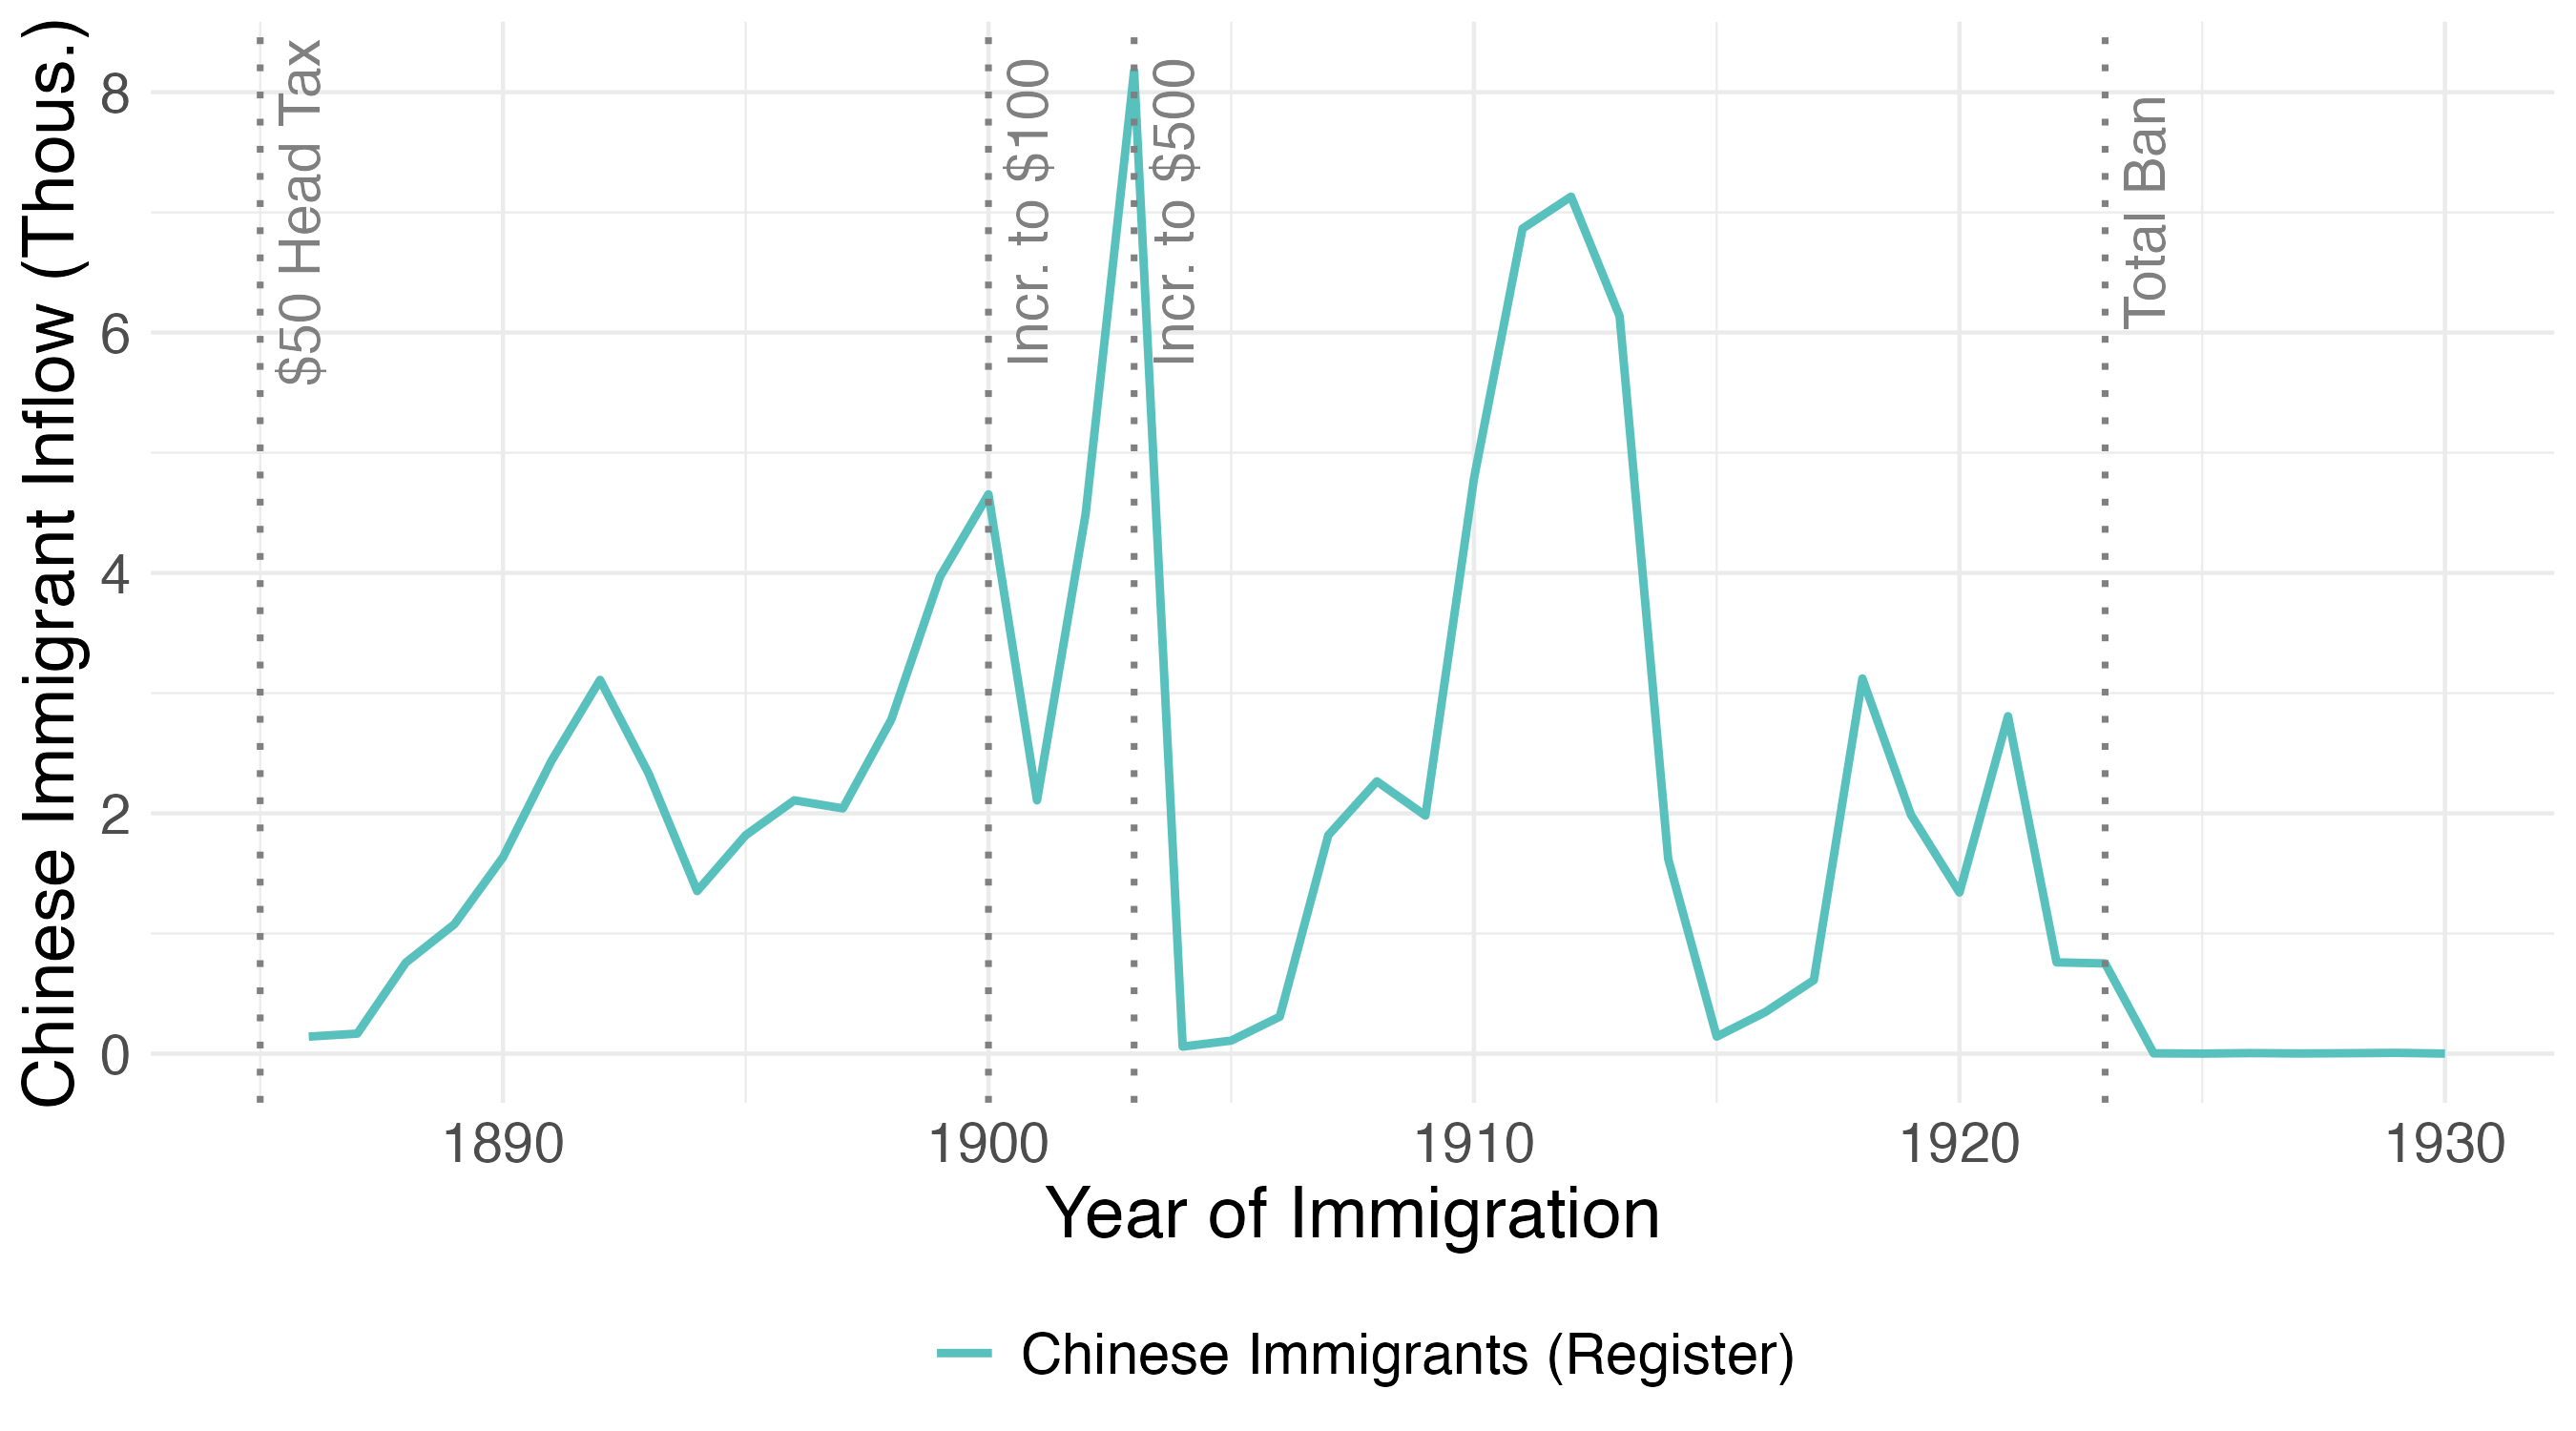
\includegraphics[width = 0.9\textwidth]{../../figs/slides/fig1_immflow_chionly.png}
    \end{figure}
\end{frame}

\begin{frame}
    \label{fig1_main}
    \frametitle{No corresponding $\Delta$ in total immigration \hyperlink{fig1_census}{\beamergotobutton{Census Data}}}
    \begin{figure}
        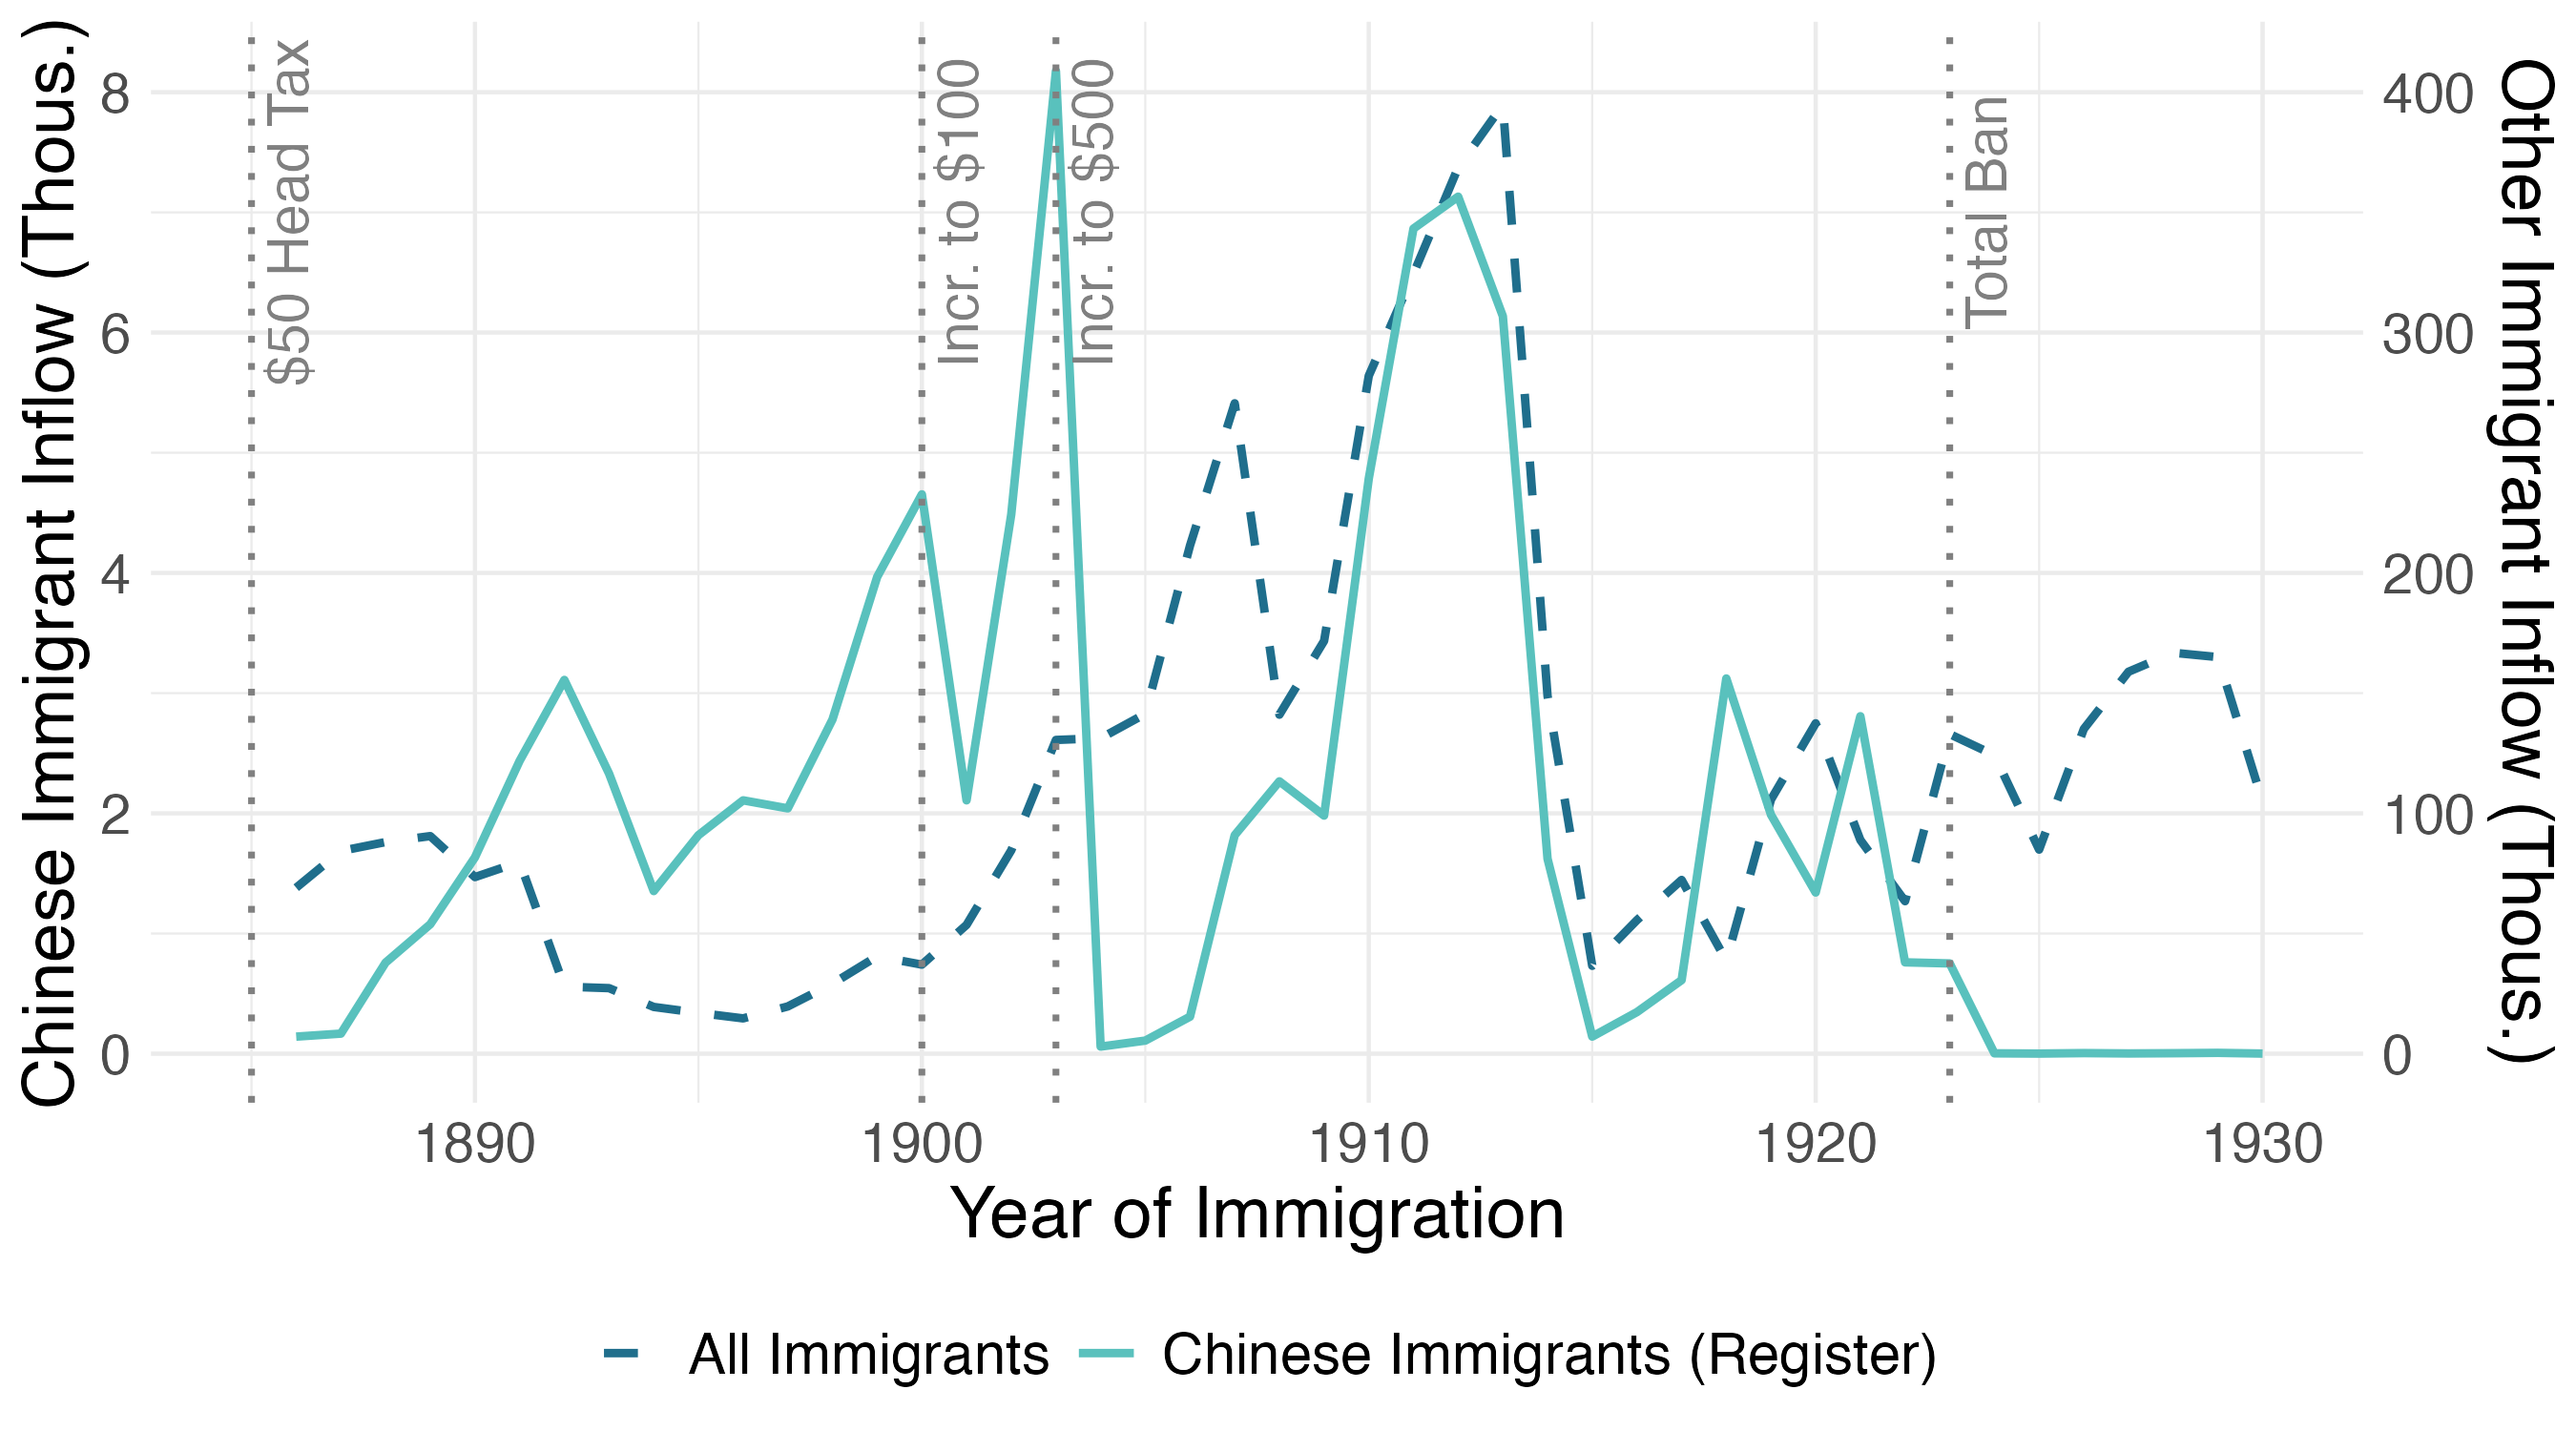
\includegraphics[width = 0.9\textwidth]{../../figs/slides/fig1_immflow.png}
    \end{figure}
\end{frame}

\begin{frame}
    \frametitle{Regression specification}
    Following similar migration analysis by Clark, Hatton and Williamson (2007):
    \begin{equation*}
        \textcolor{red}{FLOW_{t}} = \alpha_0 + \textcolor{blue}{\sum_{\tau \in \{100, 500\}} \gamma_{\tau} \mathbbm{1}[TAX_t = \tau]} + \alpha_1 HK_t + \alpha_2 CA_t + \alpha_3 P_{t-1} + \alpha_4(P_{t-1})^2
    \end{equation*}
    where
    \begin{itemize}
        \item \textcolor{red}{$FLOW_t$} is \# Chinese immigrants to Canada in year $t$ (Register)
        \item \textcolor{blue}{$TAX_t$} represents the Head Tax amount in year $t$
        \begin{itemize}
            \item \textcolor{blue}{$\gamma_{\tau}$} represents the effect of Head Tax $\tau$ relative to \$50 Tax 
        \end{itemize}
        \item Controls: 
        \begin{itemize}
            \item $HK_t$: Total emigration from Hong Kong in year $t$
            \item $CA_t$: Total immigration to Canada in year $t$
            \item $P_{t-1}$: Lagged population stock of Chinese immigrants living in Canada
        \end{itemize}
    \end{itemize}
\end{frame}

\begin{frame}
    \label{reg_flow}
    \frametitle{8.8k/year $\downarrow$ in Chinese imm. under \$500 Head Tax}
    \centering
    \begin{table}
        \resizebox{0.7\textwidth}{!}{
% Table created by stargazer v.5.2.3 by Marek Hlavac, Social Policy Institute. E-mail: marek.hlavac at gmail.com
% Date and time: Wed, Jan 17, 2024 - 11:02:36
\begin{tabular}{@{\extracolsep{5pt}}lcc} 
\\[-1.8ex] & Register (1886-1923) & Census (1880-1920) \\ 
\hline \\[-1.8ex] 
 $\gamma_{50}$ (\$50 Tax) &  & $-$411.60 (318.60) \\ 
  $\gamma_{100}$ (\$100 Tax) & $-$1,394.00 (899.20) & $-$724.90 (569.20) \\ 
  $\gamma_{500}$ (\$500 Tax) & $-$8,803.00$^{***}$ (1,210.00) & $-$1,864.00$^{**}$ (684.90) \\ 
 \hline \\[-1.8ex] 
Dep. Var. Mean & 2460.8 & 1095.4 \\ 
Observations & 36 & 41 \\ 
Adjusted R$^{2}$ & 0.75 & 0.69 \\ 
\end{tabular} 
}
    \end{table}
    \hyperlink{flow_cf}{\beamergotobutton{Counterfactual Imm.}} \hyperlink{flow_placebo1}{\beamergotobutton{Placebo Test}}
\end{frame}

%%%%%%%%%%%%%%%%%%%%%%%%%%%
%%%% Selection Effects
%%%%%%%%%%%%%%%%%%%%%%%%%%%
\section{Effects on Selection into Immigration}

\begin{frame}
    \label{theory_main}
    \frametitle{Selection: Theoretical Framework \hyperlink{theory1}{\beamergotobutton{Details}}}
    Lower returns to skill in Canada for Chinese imm $\implies$ low-skilled imm. (neg. selection) \textcolor{gray}{Chancel and Piketty 2021; 1901 Census} \vspace{2mm}
    \begin{enumerate}
        \item \textbf{Roy-Borjas}: homogeneous cost of migration \vspace{2mm}
        \begin{itemize}
            \item Supported by majority of historical immigration research \vspace{1mm}
            \item Prediction: increase in migration costs $\implies$ more \textbf{negative selection} \vspace{2mm}
        \end{itemize}
        \item \textbf{Chiquiar-Hanson}: skill-varying cost of migration  \vspace{2mm}
        \begin{itemize}
            \item More recent model to explain more positive selection from Mexico \vspace{1mm}
            \item Prediction: increase in migration costs $\implies$ more \textbf{positive selection}
        \end{itemize}
    \end{enumerate}
\end{frame}

\begin{frame}
    \frametitle{Measuring Selection in the Chinese Register}
    \textbf{Height} \vspace{2mm}
    \begin{itemize}
        \item Recorded by officials at time of arrival for all Chinese immigrants \vspace{2mm}
        \item After age ~23, independent of decision to migrate -- common metric of human capital  \vspace{2mm}
        \item Can compare with existing estimates of height of Chinese population \vspace{2mm}
    \end{itemize}
\end{frame}

\begin{frame}
    \frametitle{Increase in Chinese Immigrant Height as HT $\uparrow$...}
    \begin{figure}
        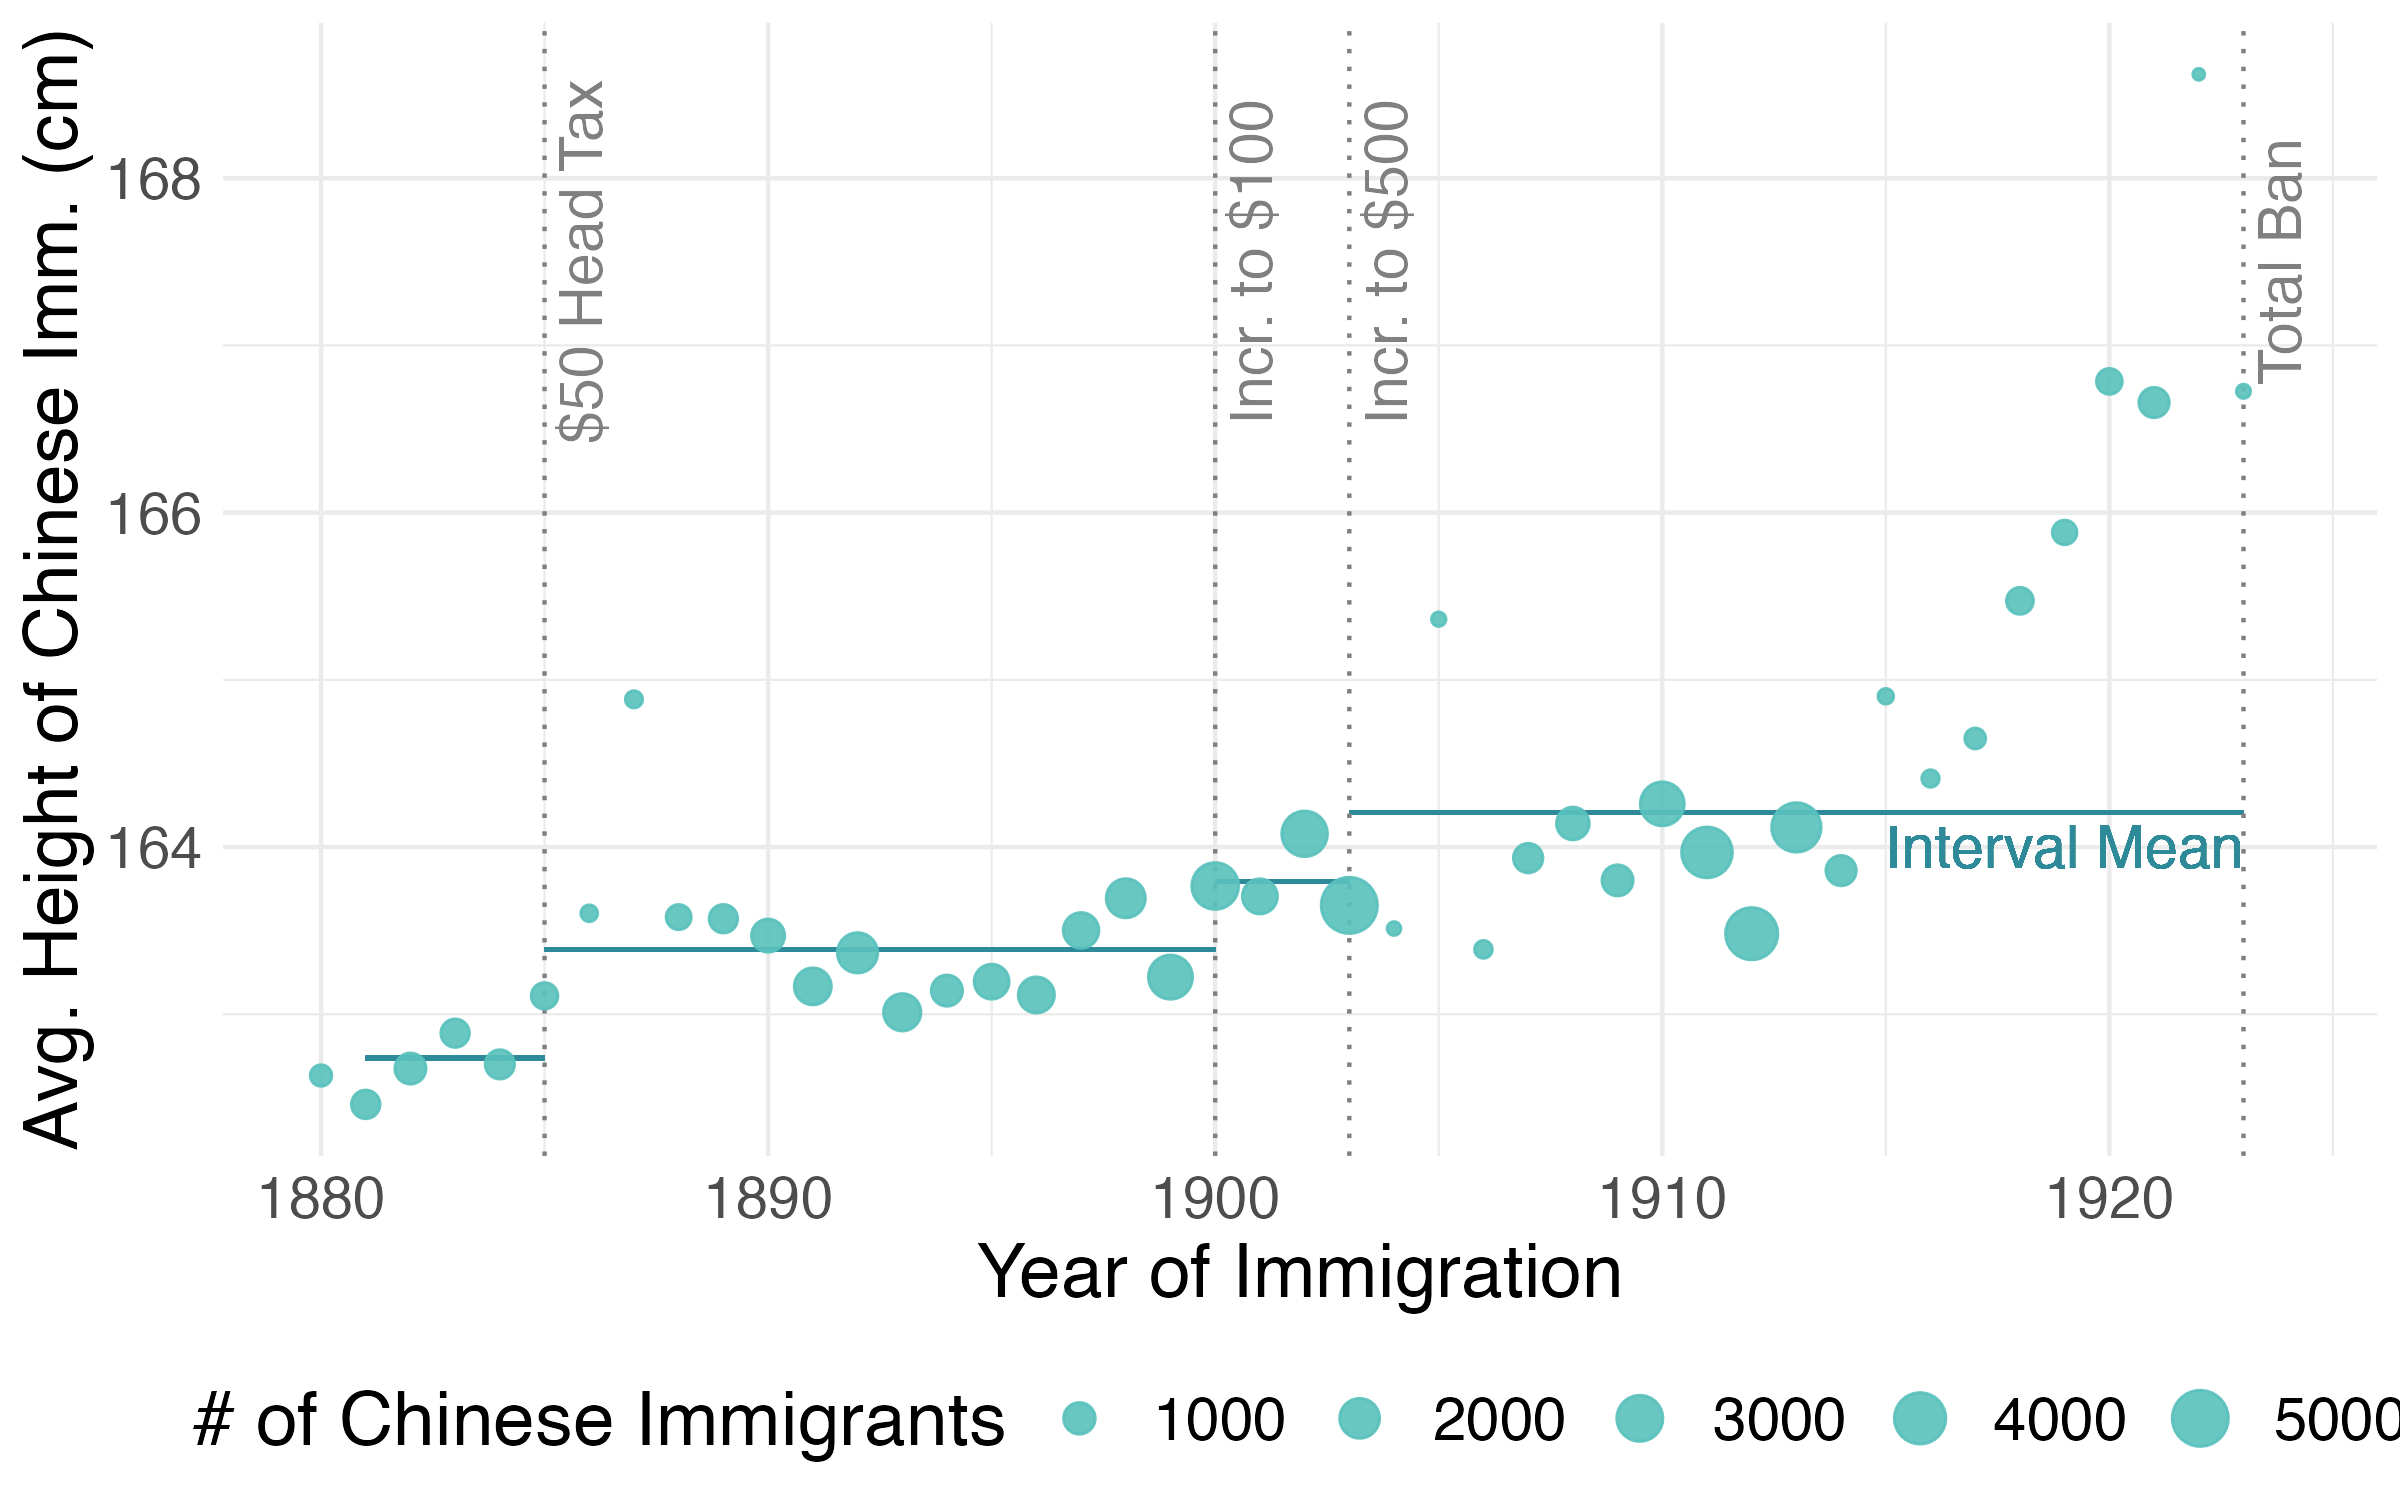
\includegraphics[width = 0.8\textwidth]{../../figs/slides/height_selection.png}
    \end{figure}
\end{frame}

\begin{frame}
    \label{height2}
    \frametitle{...especially relative to Chinese population \hyperlink{baten_graph}{\beamergotobutton{Other Height Samples}}}
    \begin{figure}
        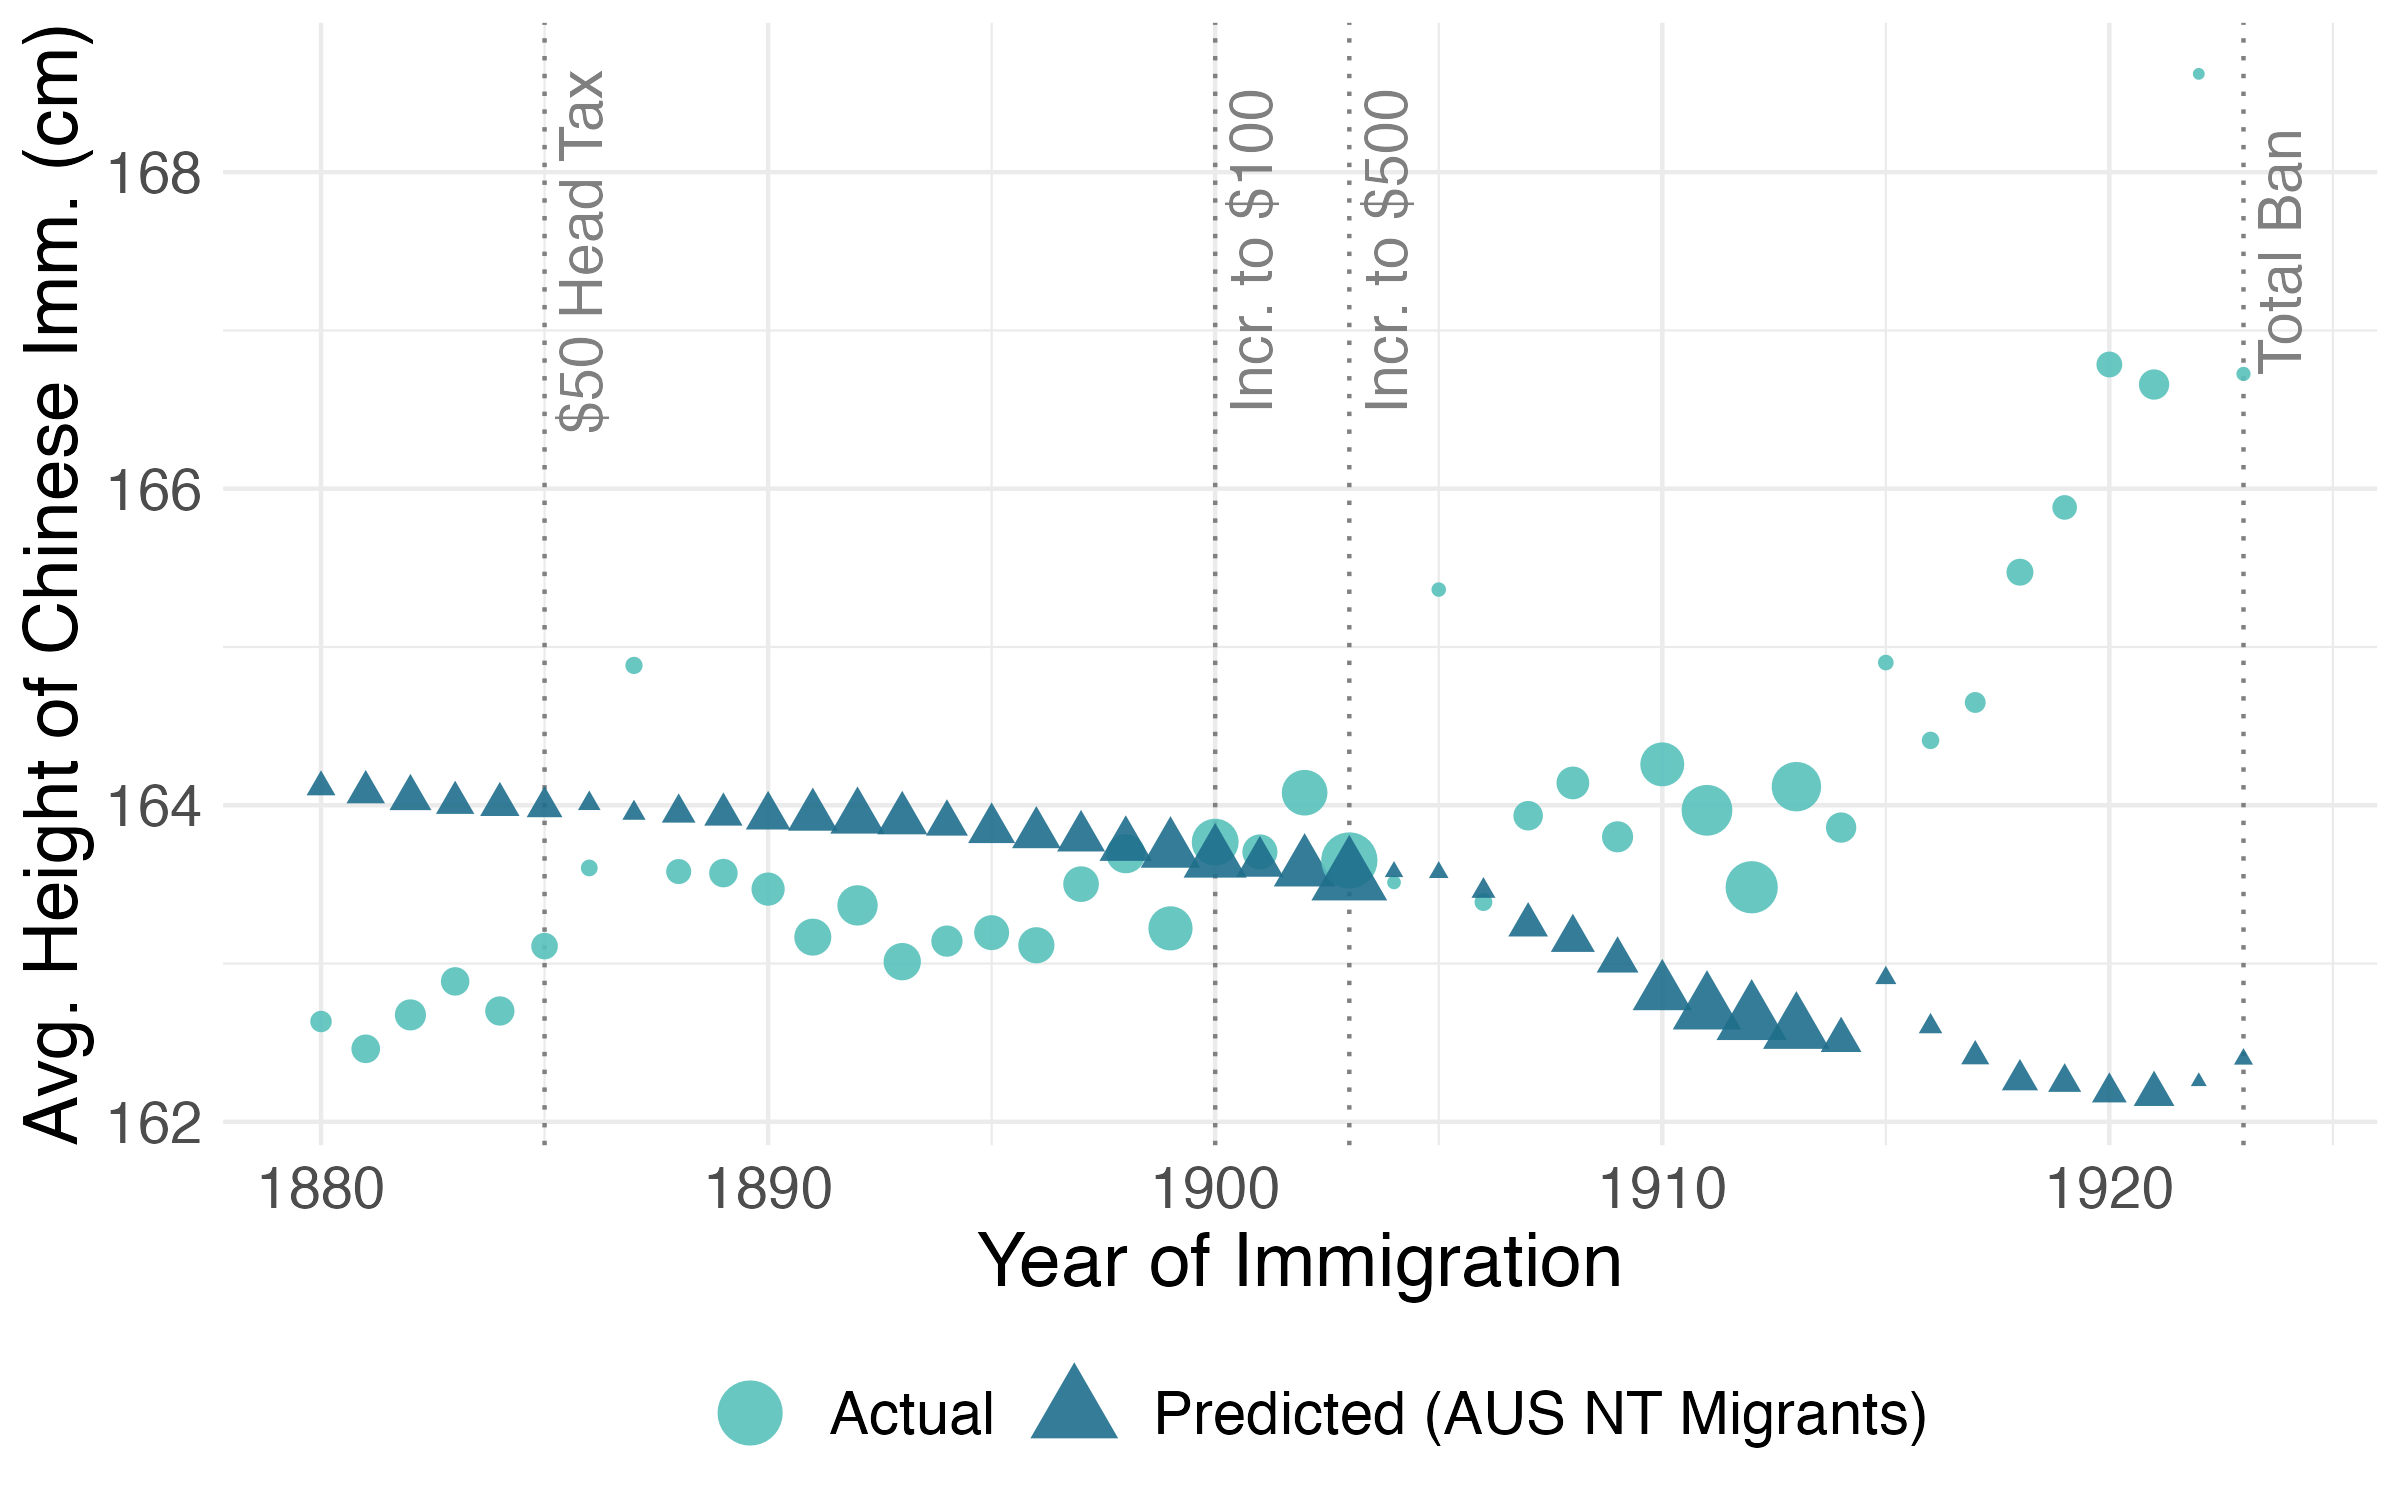
\includegraphics[width = 0.8\textwidth]{../../figs/slides/height_compare_selection.png}
    \end{figure}
\end{frame}

\begin{frame}
    \frametitle{Measuring Selection in the Census}
    \textbf{Occupation, Literacy, Home Ownership} \vspace{2mm}
    \begin{itemize}
        \item Biased by return migration \& post-arrival factors \vspace{2mm}
        \item \textbf{But} can compare with other immigrants as `counterfactual'  \vspace{2mm}
        \item Can rule out `Canada-wide' effect 
    \end{itemize}
\end{frame}

\begin{frame}
    \frametitle{Empirical Specification: Standard Difference-in-Differences}
    \begin{equation*}
        \label{eq:did}
        \textcolor{red}{y_{ict}} = \beta_1 C_i + \beta_2 A_{ic} + \delta_c + \delta_t + \textcolor{blue}{\sum_{\tau \in \{50,100,500\}} \gamma_\tau^{DD} \times C_i \times \mathbf{1}[TAX_t = \tau]}  + \varepsilon_{ict}
    \end{equation*}
    \begin{itemize}
        \item \textcolor{red}{$y_{ict}$} is the outcome of interest for individual $i$ as measured in census year $c$, who immigrated to Canada in year $t$
        \item $C_i$ is an indicator for $i$ having been born in China 
        \item $A_{ic}$ is a control for age 
        \item $\delta_c$ and $\delta_t$ are census year and arrival year FEs respectively  
        \item As before, \textcolor{blue}{$TAX_t$} represents the Head Tax amount in year $t$
        \begin{itemize}
            \item \textcolor{blue}{$\gamma_{\tau}^{DD}$}: effect of HT $\tau$ rel. to no tax for Chinese rel. to non-Chinese imm. 
        \end{itemize}
    \end{itemize}
    \textbf{ID Assumption:} Without the Head Tax, characteristics of Chinese and non-Chinese imm. would have evolved in parallel
\end{frame}

\begin{frame}
    \label{reg_sel1}
    \frametitle{More positive selection of Chinese vs. all imm. when HT $\uparrow$}
    \centering
    \begin{table}
        \resizebox{0.9\textwidth}{!}{
% Table created by stargazer v.5.2.3 by Marek Hlavac, Social Policy Institute. E-mail: marek.hlavac at gmail.com
% Date and time: Tue, Jan 16, 2024 - 18:31:32
\begin{tabular}{@{\extracolsep{5pt}}lccc} 
\\[-1.8ex]\\[-1.8ex] & $\mathbb{P}[\text{Laborer}]$ & $\mathbb{P}[\text{Literate}]$ & $\mathbb{P}[\text{Owns House}]$ \\ 
\hline \\[-1.8ex] 
 $\hat{\beta}_{1}$ (Born in China) & 0.252$^{***}$ (0.032) & $-$0.396$^{***}$ (0.024) & $-$0.497$^{***}$ (0.038) \\ 
  $\hat{\gamma}_{50}^{DD}$ ($C_i \times$ \$50 Tax) & $-$0.038 (0.035) & 0.181$^{***}$ (0.027) & 0.101$^{**}$ (0.041) \\ 
  $\hat{\gamma}_{100}^{DD}$ ($C_i \times$ \$100 Tax) & 0.035 (0.039) & 0.200$^{***}$ (0.029) & 0.014 (0.046) \\ 
  $\hat{\gamma}_{500}^{DD}$ ($C_i \times$ \$500 Tax) & $-$0.132$^{***}$ (0.034) & 0.120$^{***}$ (0.026) & 0.133$^{***}$ (0.040) \\ 
 \hline \\[-1.8ex] 
Dep. Var. Mean (Chinese) & 0.3582 & 0.6715 & 0.1325 \\ 
Observations & 55,149 & 56,156 & 57,148 \\ 
Adjusted R$^{2}$ & 0.062 & 0.050 & 0.123 \\ 
\end{tabular} 
}
    \end{table}
    \hyperlink{reg_sel2}{\beamergotobutton{Japanese Imm Only}}
\end{frame}


%%%%%%%%%%%%%%%%%%%%%%%%%%%
%%%% Conclusion
%%%%%%%%%%%%%%%%%%%%%%%%%%%
\section{Conclusion}
\begin{frame}
    \frametitle{Summary of Results}
    \begin{itemize}
        \item Direct negative impact of Head Tax on level of Chinese immigration to Canada \vspace{2mm}
        \item Chinese immigrants more positively selected on height as Head Tax increased \vspace{2mm}
        \item More positively selected on occupation, literacy, home ownership vs. all other immigrants, only on occupation rel. to Japanese immigrants as HT $\uparrow$ \vspace{2mm}
        \item Results support Chiquiar-Hanson model with skill-varying migration cost  \vspace{2mm}
        \item \textbf{Takeaway:} High migration cost $\implies$ `pricing out' immigrants with most to gain  \vspace{2mm}
    \end{itemize}
\end{frame}

%%%%%%%%%%%%%%%%%%%%%%%%%%%
%%%% Appendix
%%%%%%%%%%%%%%%%%%%%%%%%%%%
\appendix 
\begin{frame}
    \label{figa1_tax}
    \frametitle{Average Non-Zero Tax Paid by Chinese Imm.  \hyperlink{headtaxinfo}{\beamerreturnbutton{Return}}}
    \centering
    \begin{figure}
        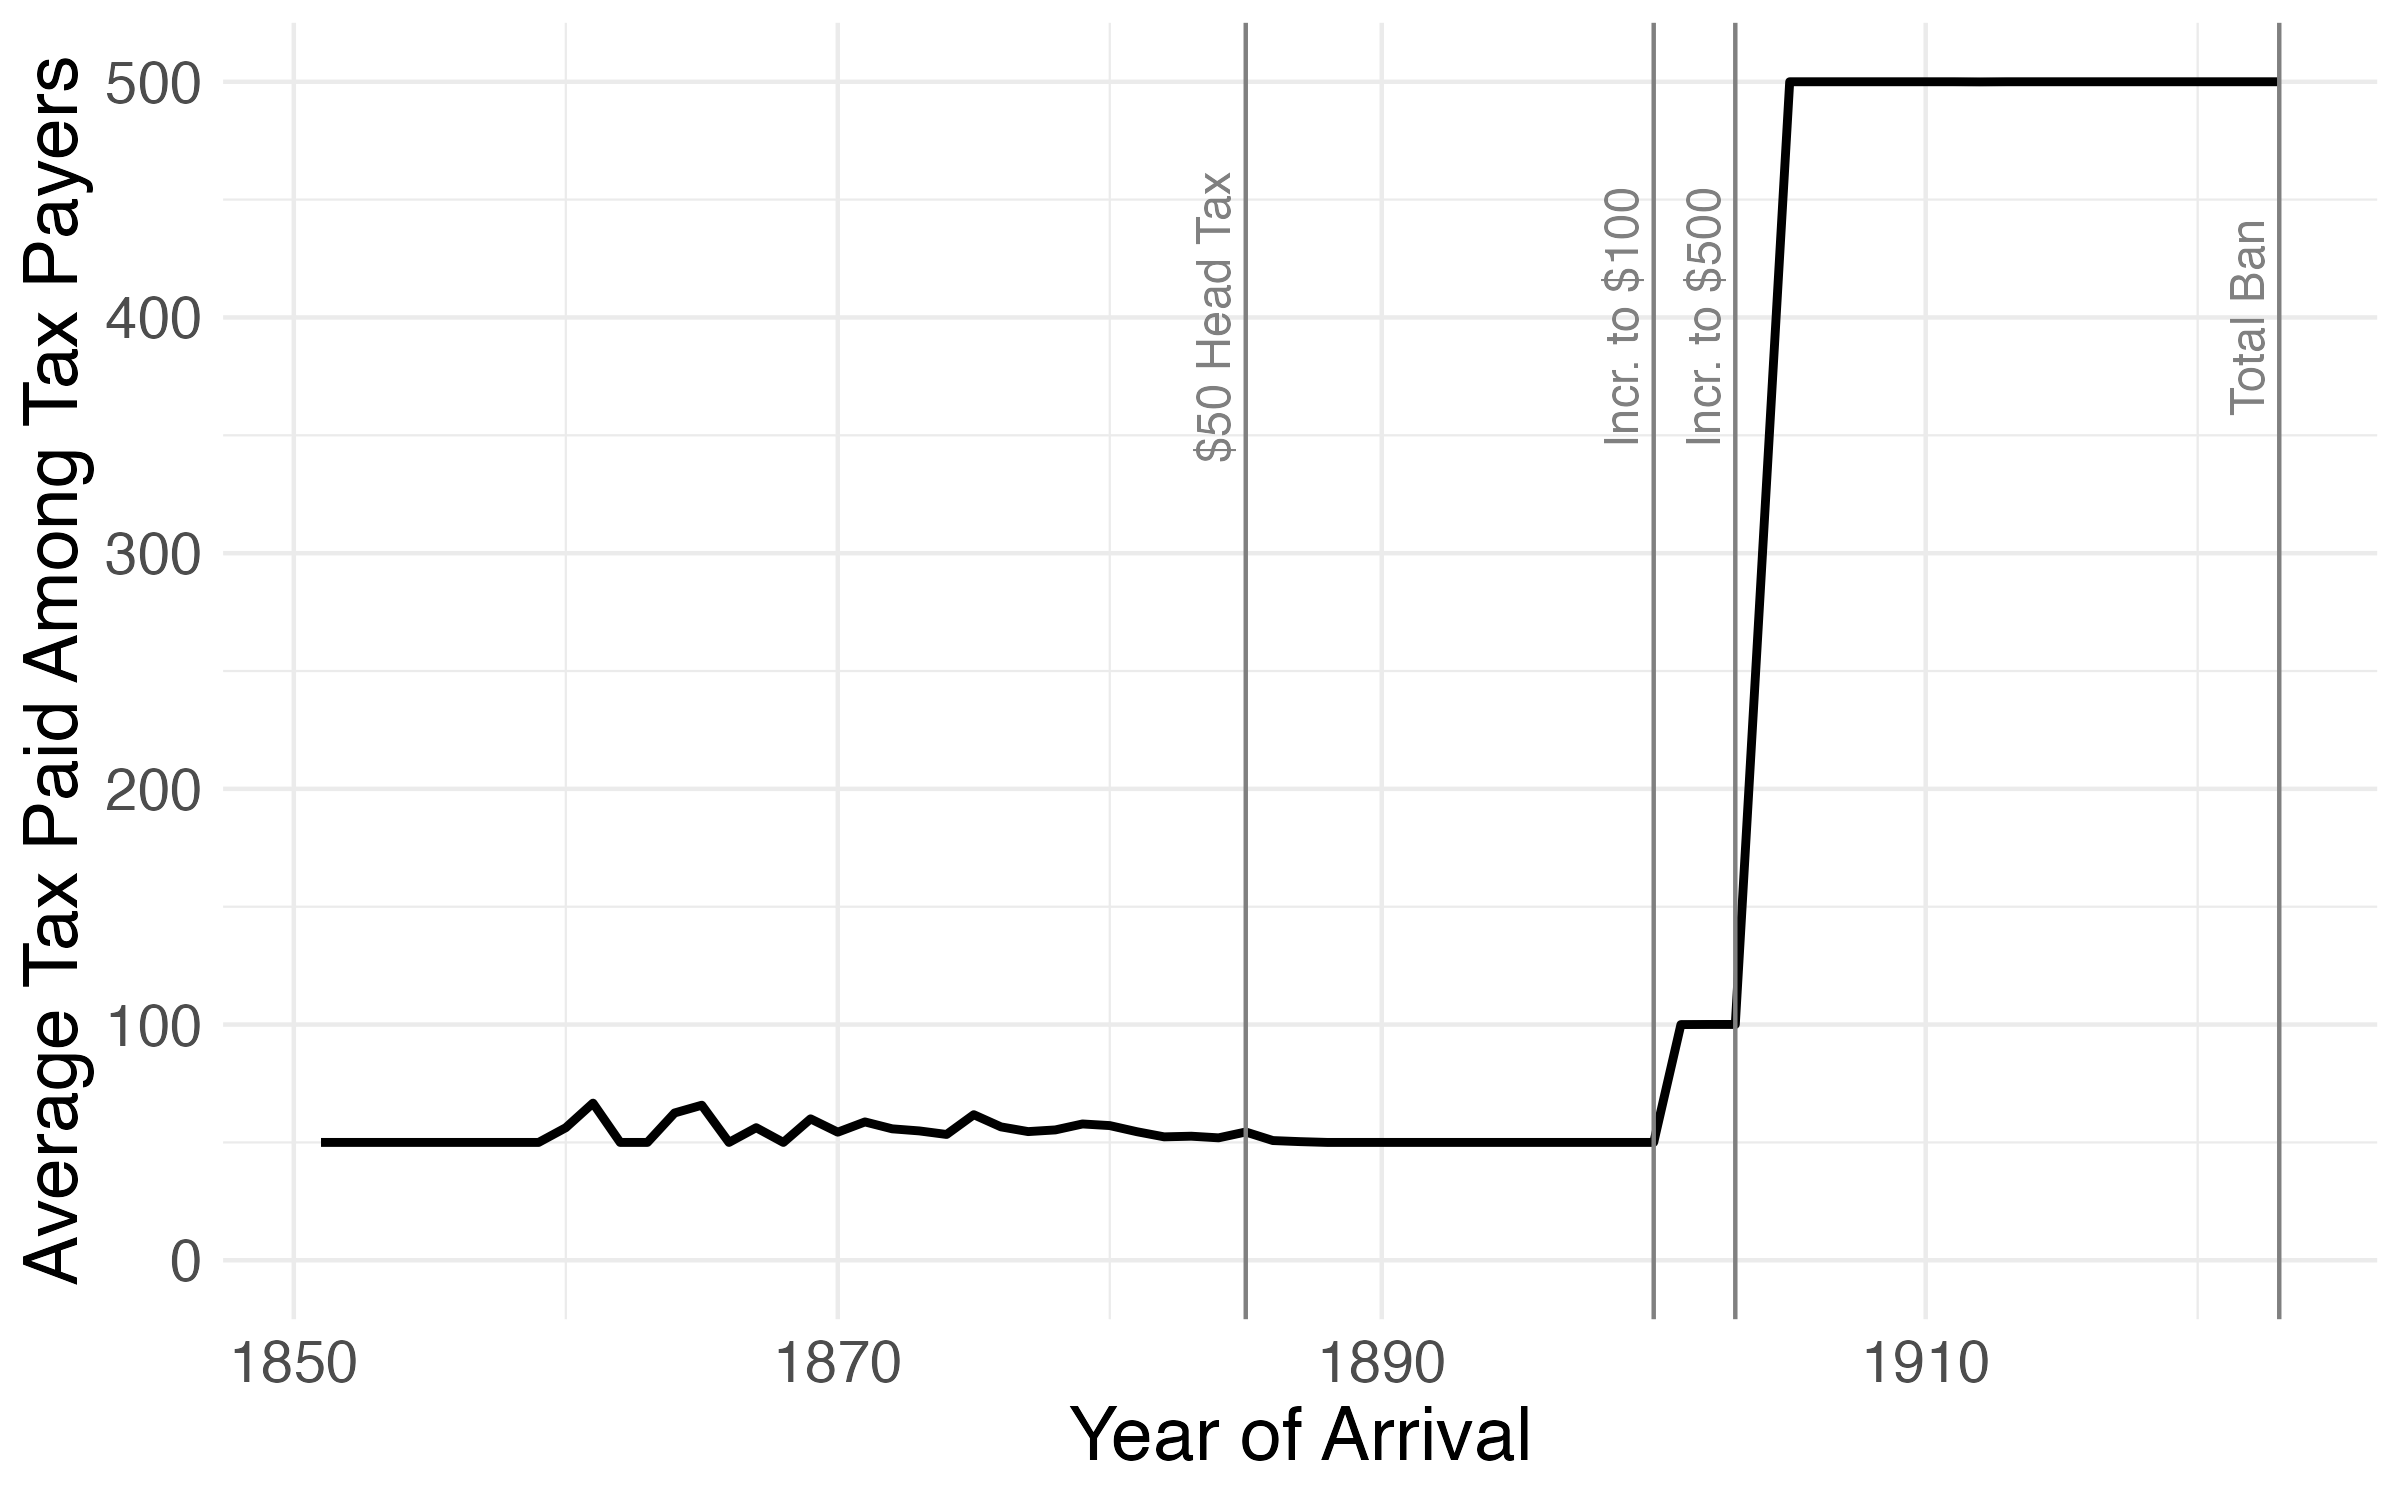
\includegraphics[width = 0.8\textwidth]{../../figs/slides/fig1_taxespaid.png}
    \end{figure}
\end{frame}

\begin{frame}
    \label{fig_headtax}
    \frametitle{Head Tax Certificate \hyperlink{headtaxinfo}{\beamerreturnbutton{Return}}}
    \centering
    \begin{figure}
        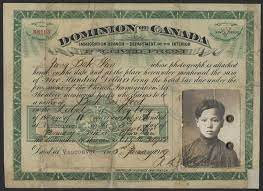
\includegraphics[width = 0.6\textwidth]{../../figs/slides/headtax.jpeg}
        \caption{\footnotesize Chinese Immigration Certificate, Library and Archives Canada (R1206-178-X-E) via The Canadian Encyclopedia}
    \end{figure}
\end{frame}

\begin{frame}
    \label{fig_register}
    \frametitle{Chinese Register  \hyperlink{data}{\beamerreturnbutton{Return}}}
    \centering
    \begin{figure}
        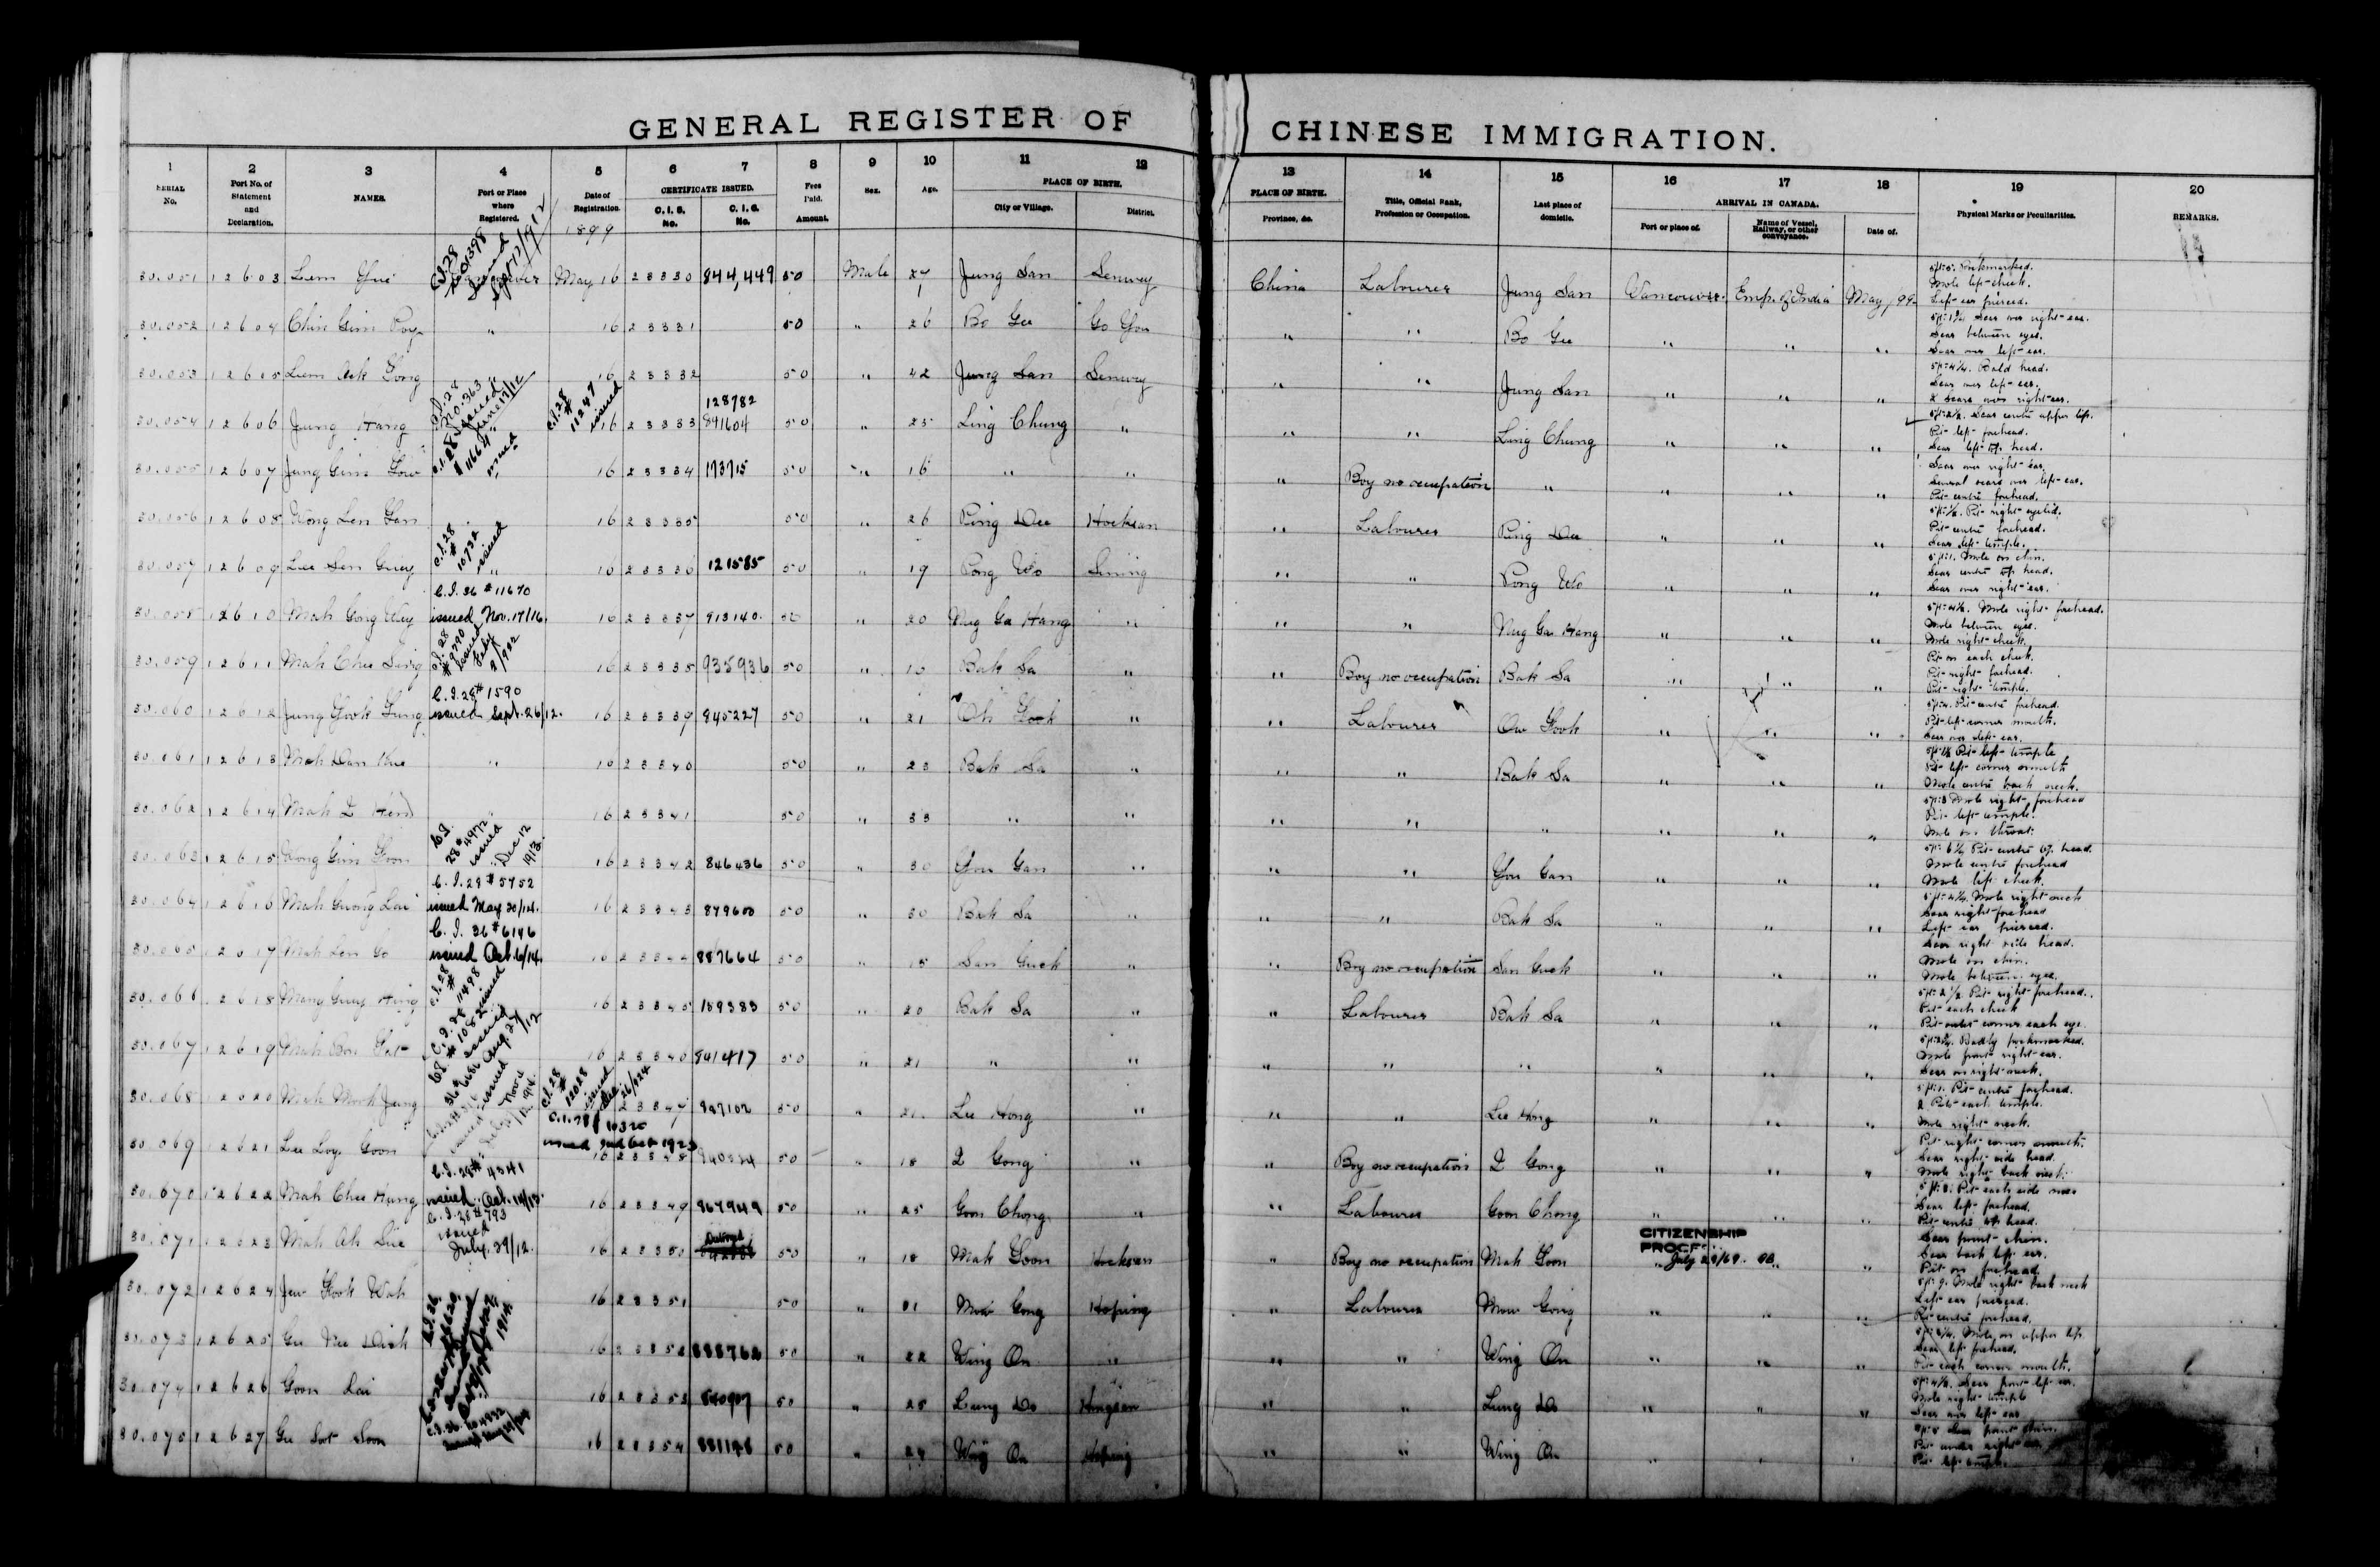
\includegraphics[width = 0.6\textwidth]{../../figs/slides/register.jpeg}
        \caption{\footnotesize General Register of Chinese Immigration, RG76, Volume 700 (e006066717) via Library and Archives Canada Blog}
    \end{figure}
\end{frame}

\begin{frame}
    \label{figa2_imm}
    \frametitle{Chinese Immigration to Canada by Data Source \hyperlink{data}{\beamerreturnbutton{Return}}}
    \centering
    \begin{figure}
        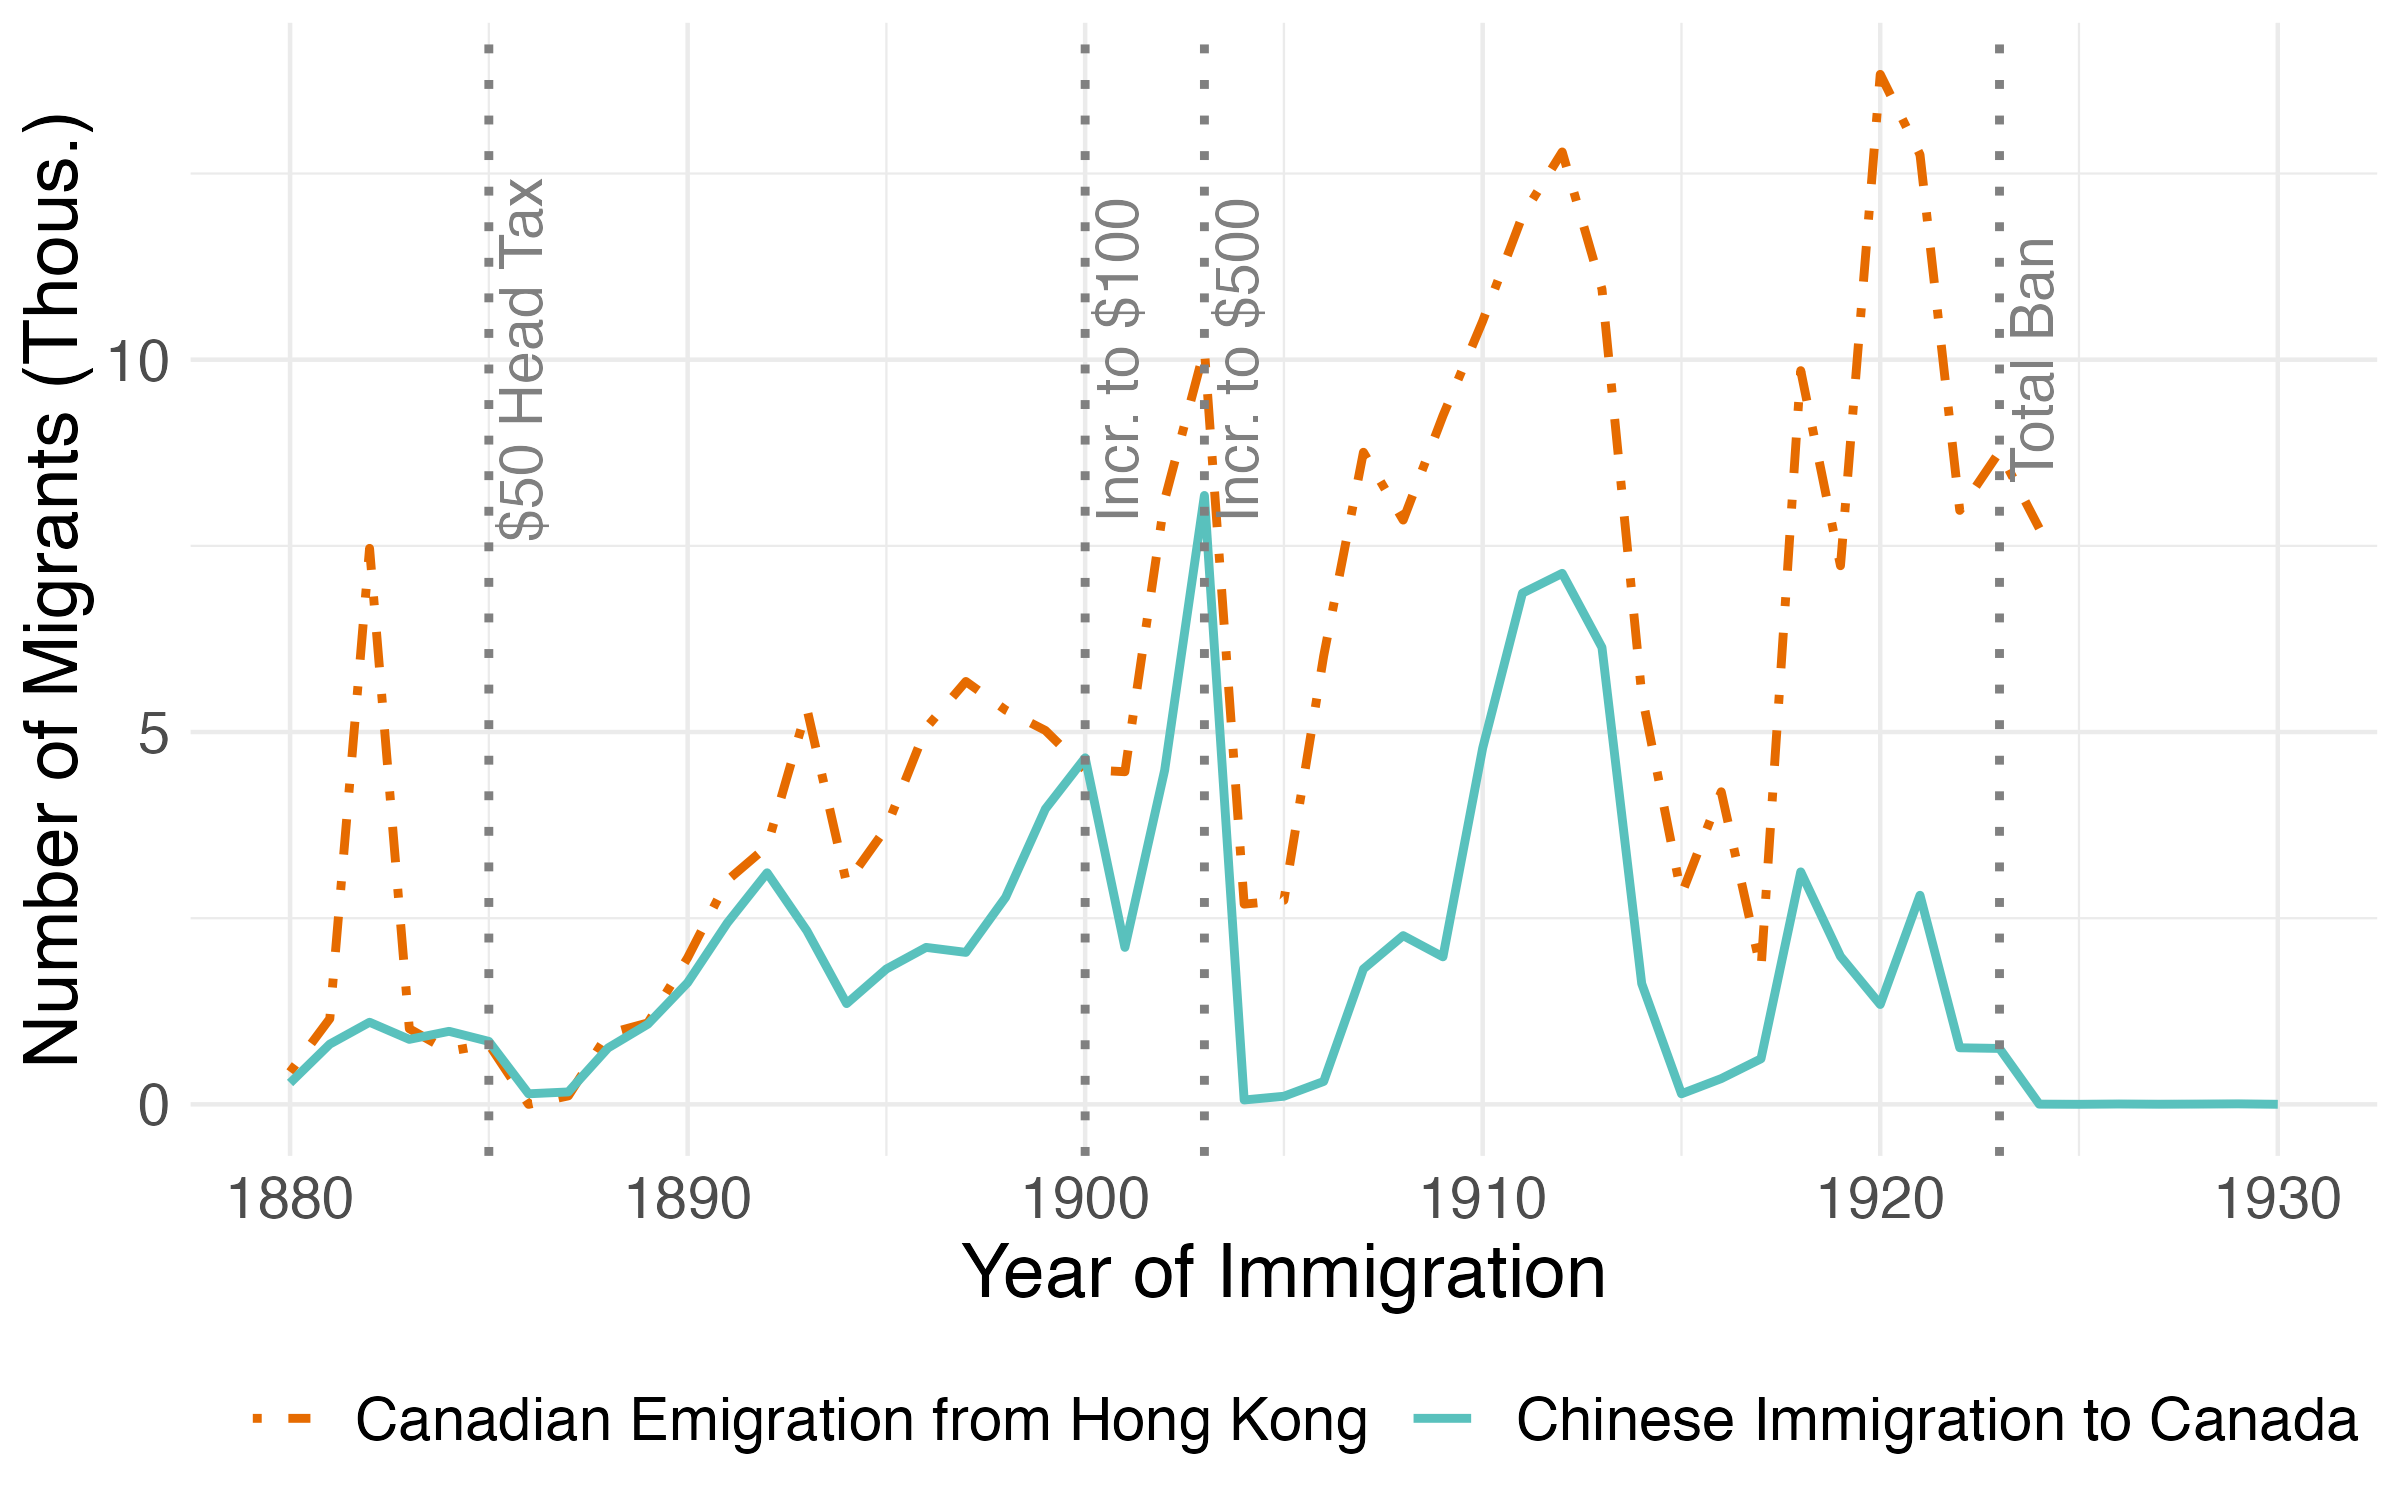
\includegraphics[width = 0.9\textwidth]{../../figs/slides/fig2_flow_immandem.png}
    \end{figure}
\end{frame}

\begin{frame}
    \label{fig1_census}
    \frametitle{Chinese vs. Total Immigration with Census Data \hyperlink{fig1_main}{\beamerreturnbutton{Return}}}
    \centering
    \begin{figure}
        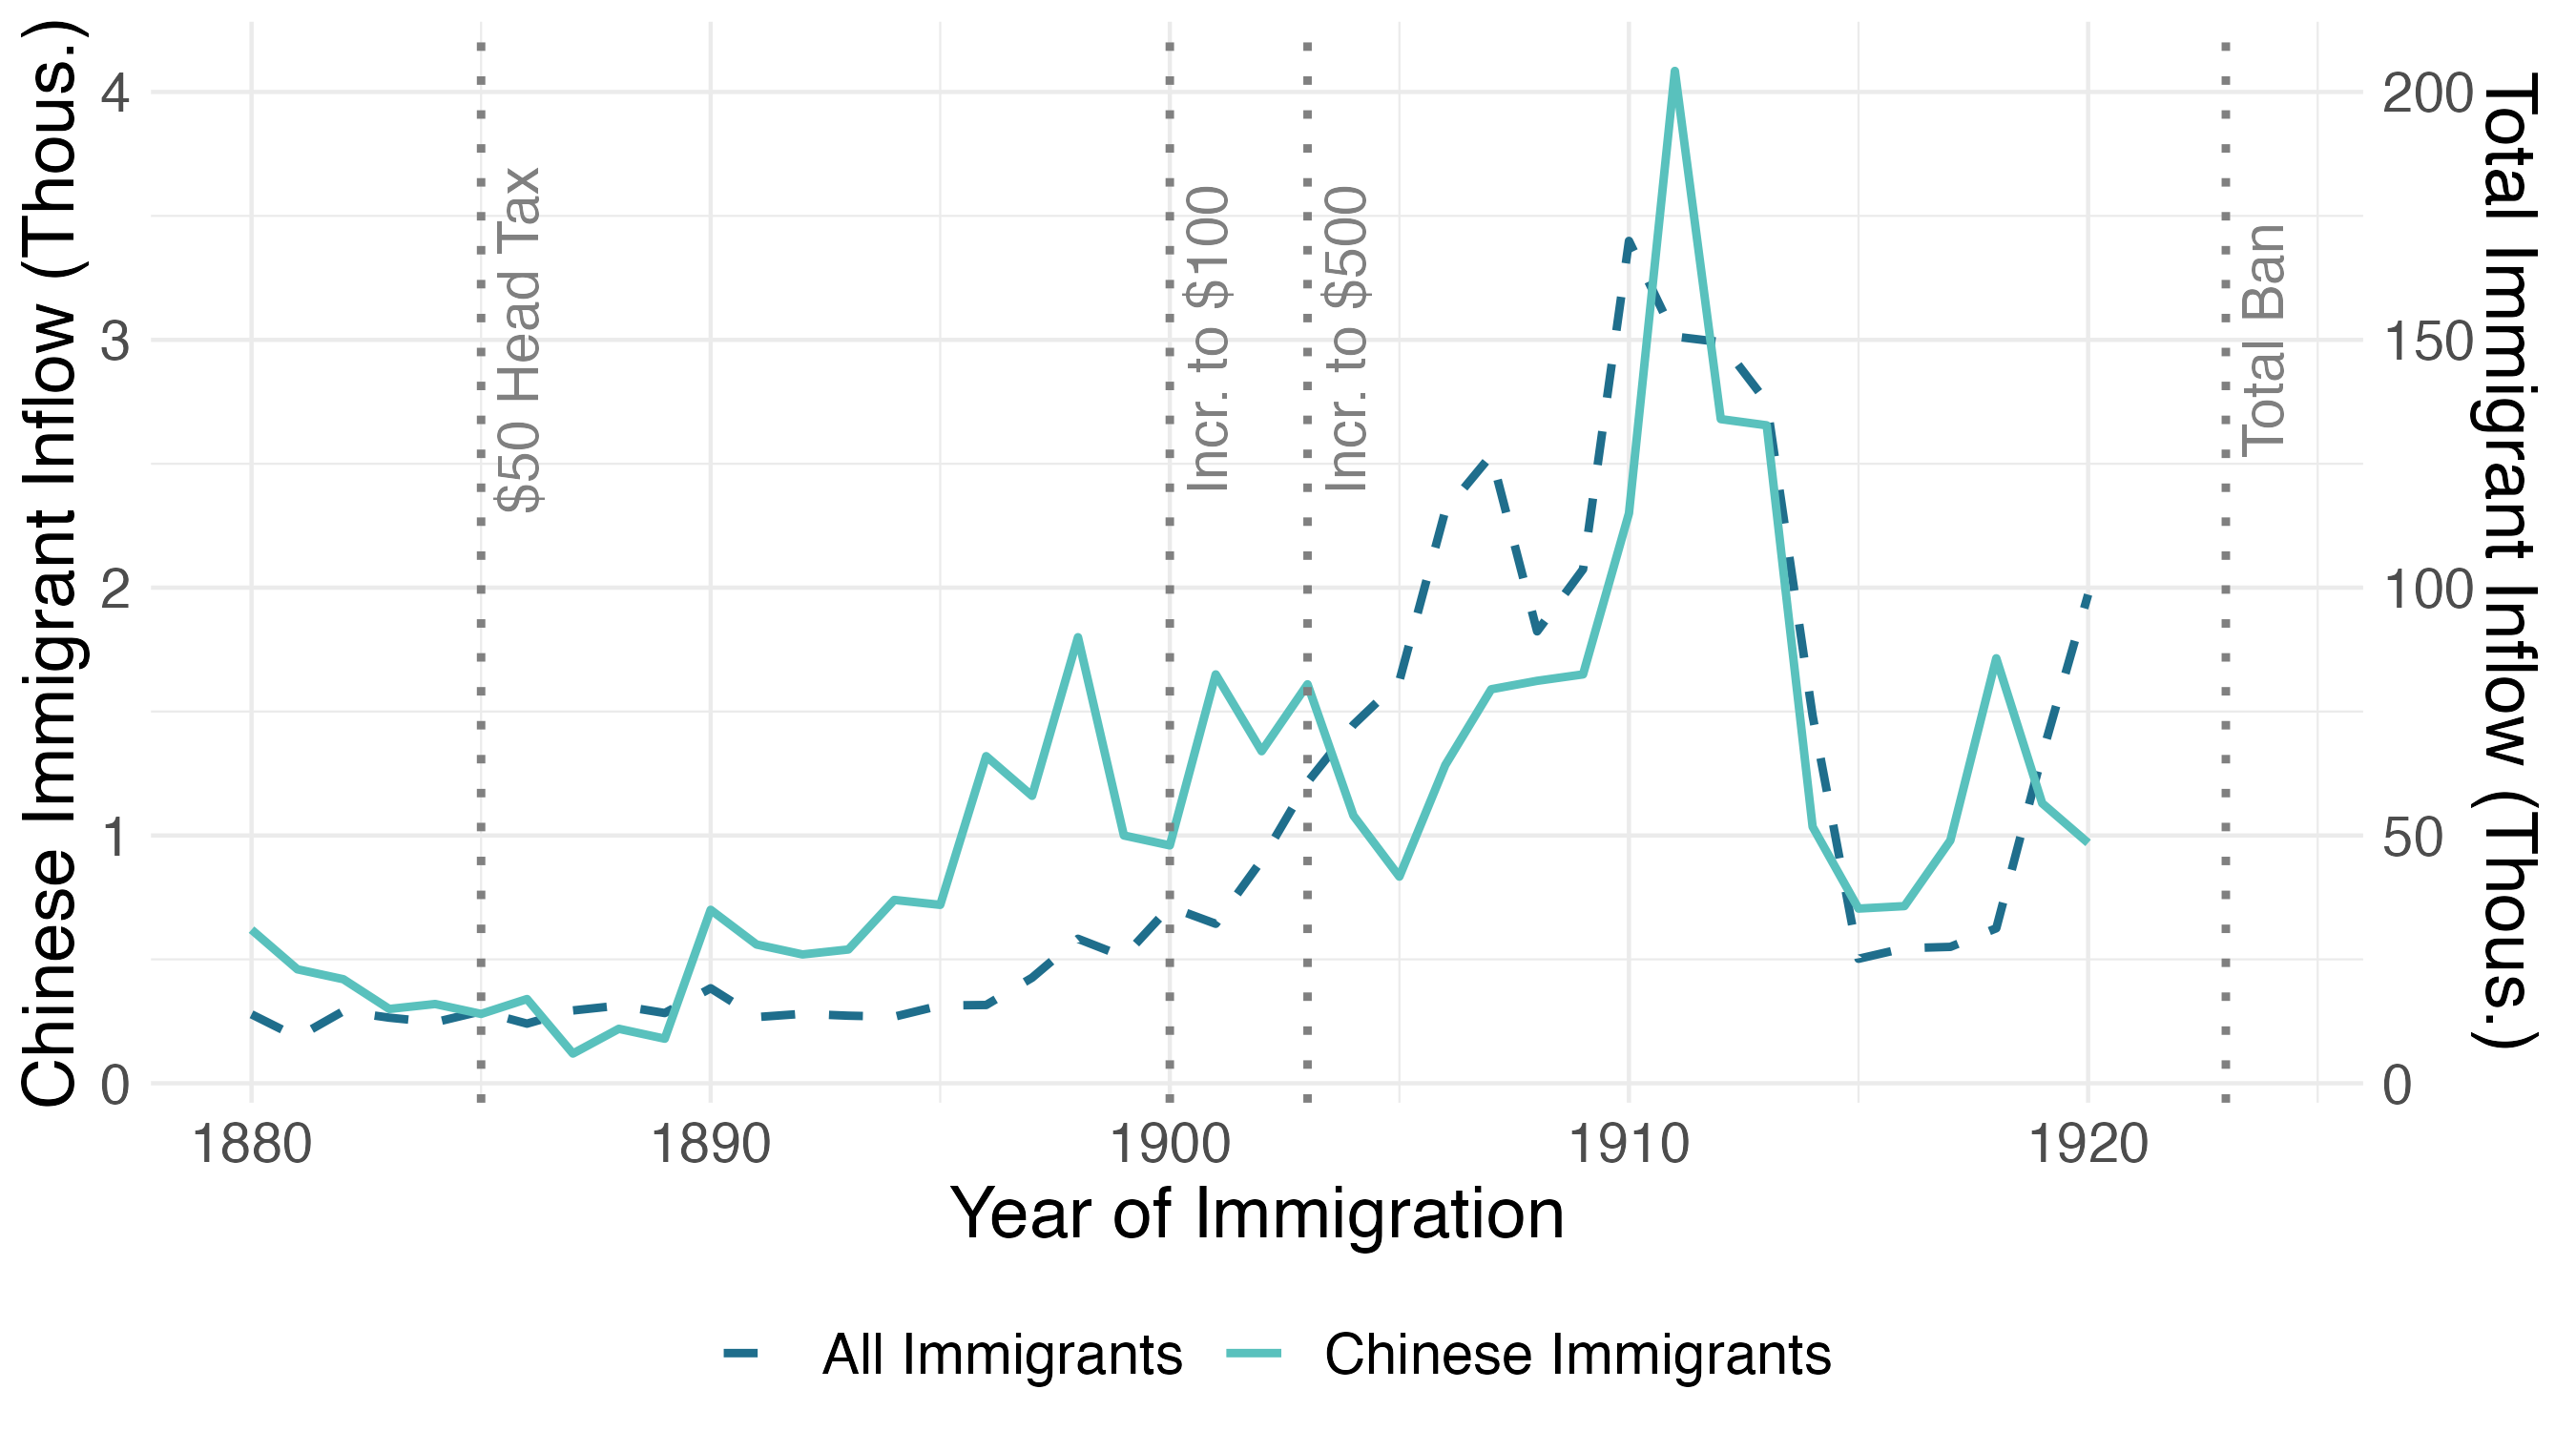
\includegraphics[width = 0.9\textwidth]{../../figs/slides/fig2_census_flow.png}
    \end{figure}
\end{frame}

\begin{frame}
    \label{flow_cf}
    \frametitle{Actual vs. Counterfactual Chinese Immigration \hyperlink{reg_flow}{\beamerreturnbutton{Return}}}
    \centering
    \begin{figure}
        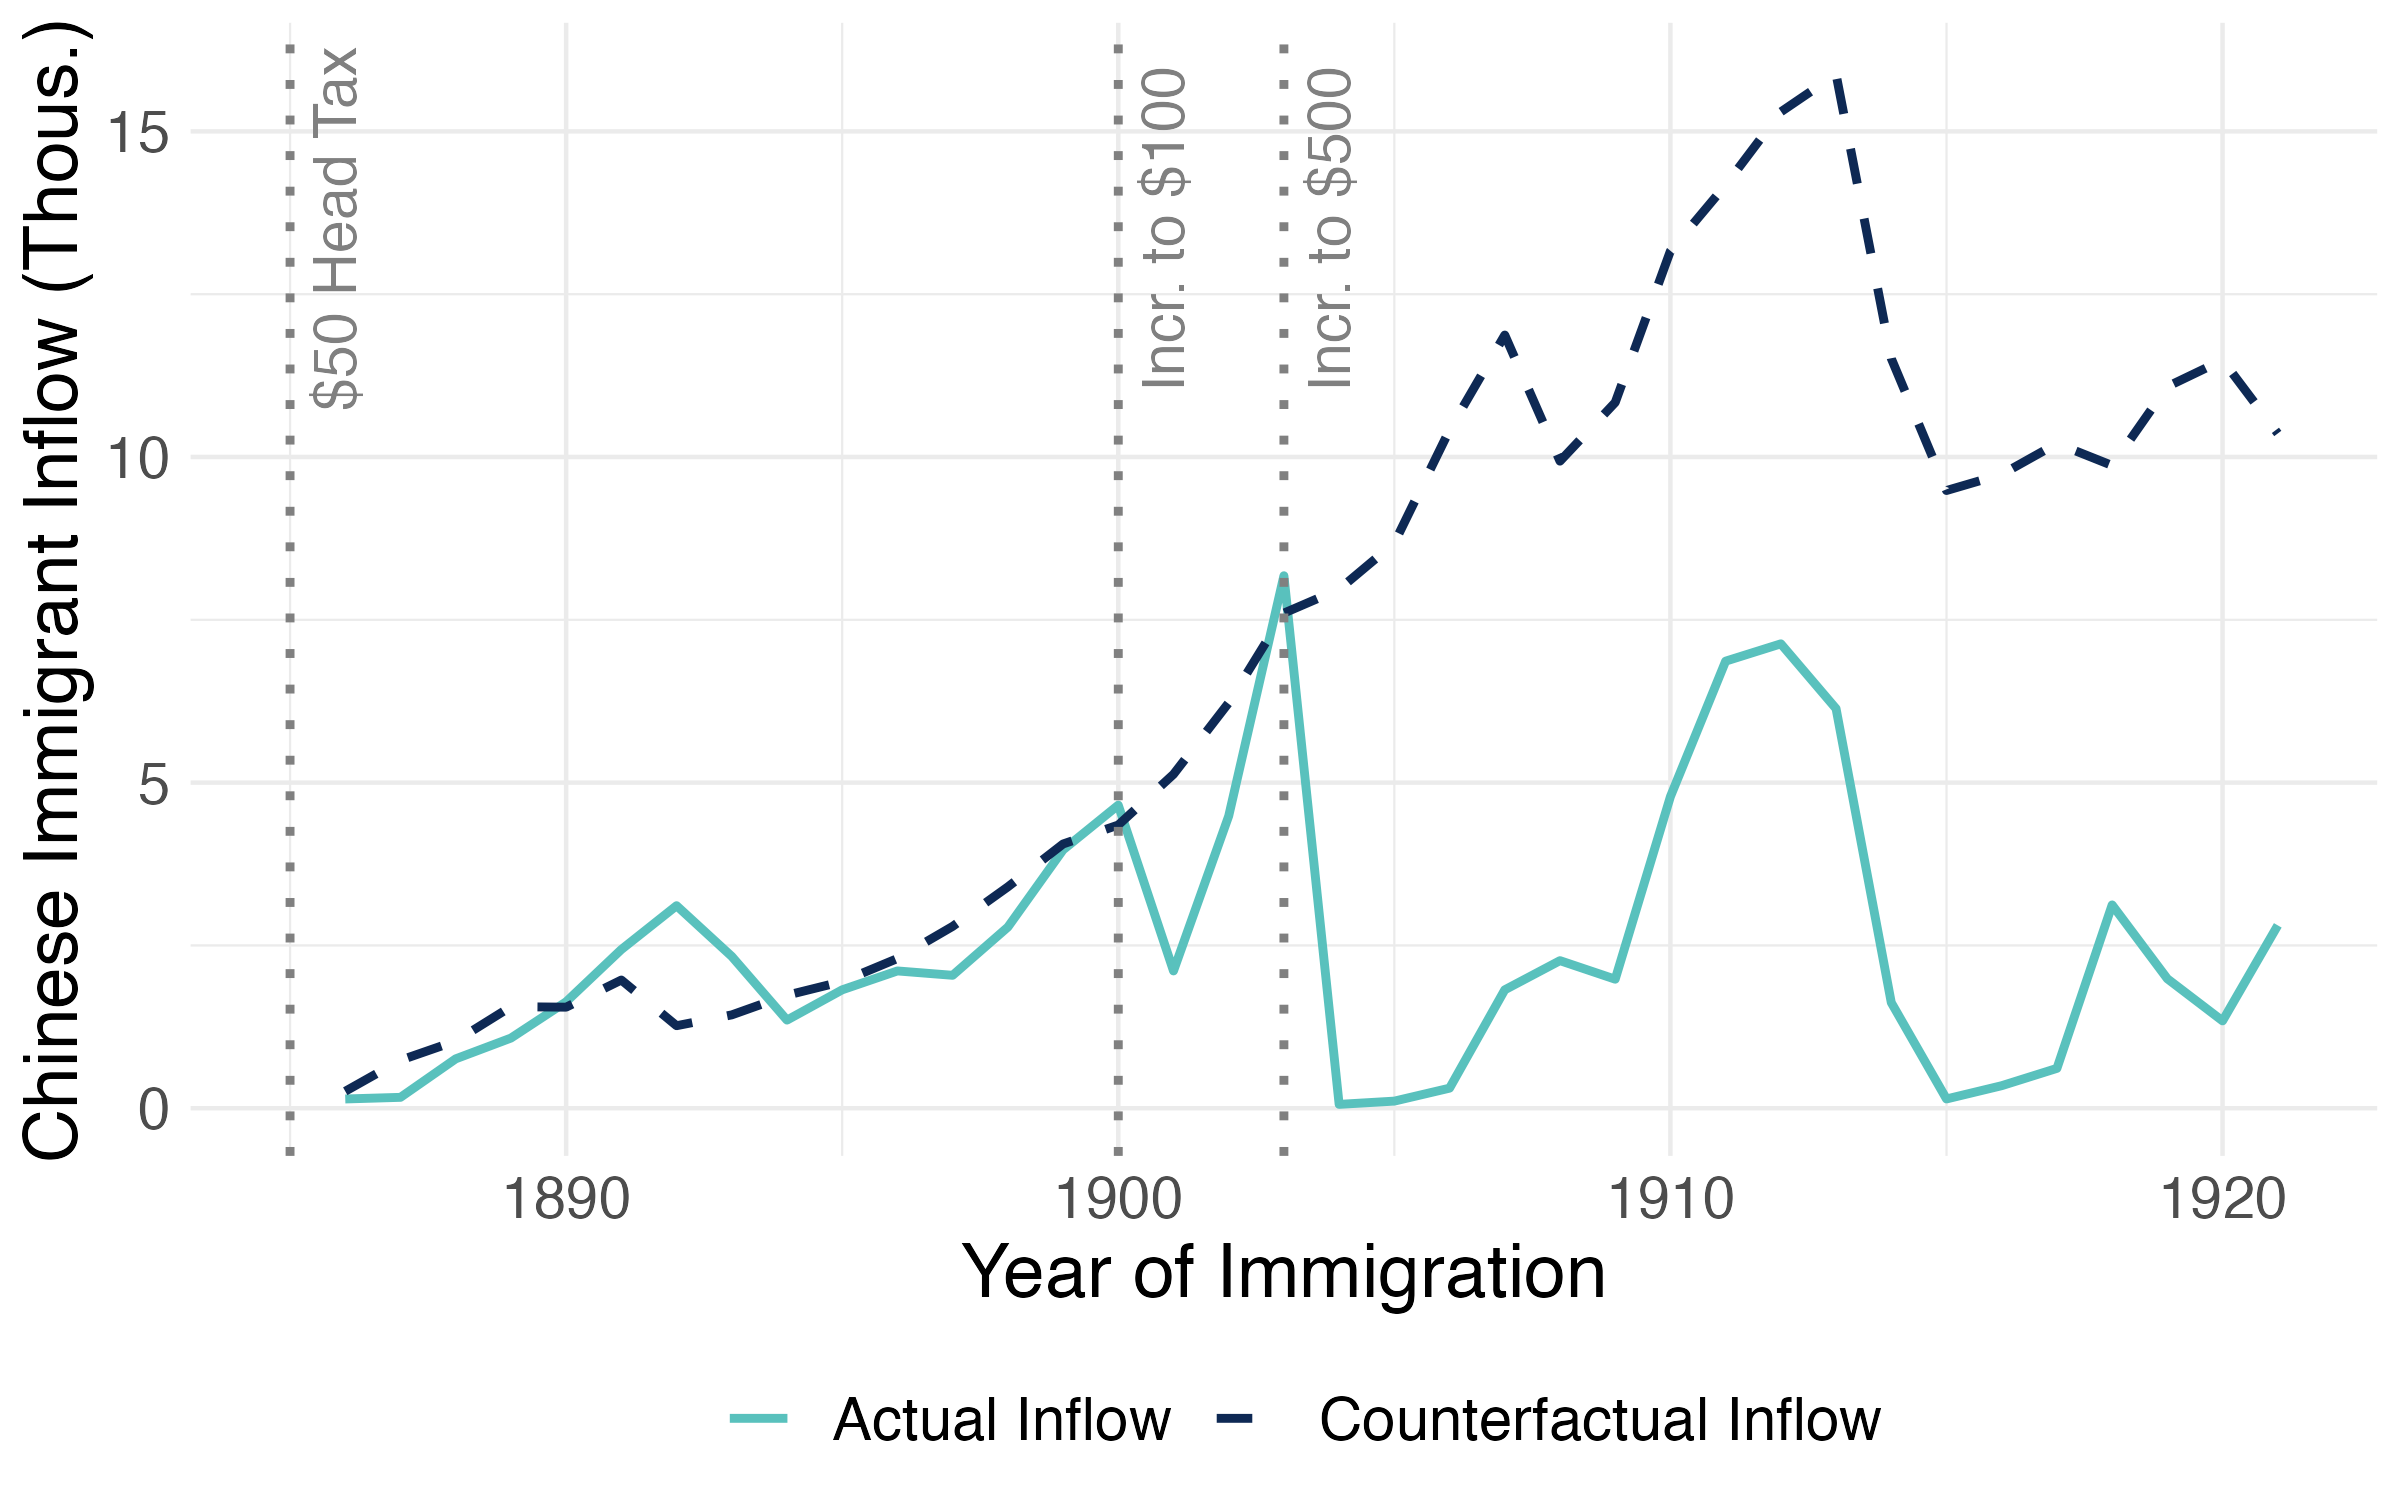
\includegraphics[width = 0.8\textwidth]{../../figs/slides/immflow_counterfactual.png}
    \end{figure}
\end{frame}

\begin{frame}
    \label{flow_placebo1}
    \frametitle{Placebo: Effects of HT on Other Countries' Imm \hyperlink{reg_flow}{\beamerreturnbutton{Return}}}
    Modifying original regression for cross-country comparison:
    \begin{equation*}
        \textcolor{red}{\log(FLOW_{ct}/POP_{ct})} = \alpha_0 + \textcolor{blue}{\sum_{\tau \in \{50, 100, 500\}} \gamma_{\tau} \mathbbm{1}[TAX_t = \tau]} + \alpha_2 CA_t + \alpha_3 P_{t-1} + \alpha_4(P_{t-1})^2
    \end{equation*}
    where $c$ indexes country and $POP_{ct}$ represents origin-country population, such that the dependent variable is now the log of the \textbf{migration rate}.
    \vspace{2mm}
    \textbf{Sample:} All countries with at least 20 years of non-zero immigration flow to Canada in the Census between 1880 and 1920.
\end{frame}

\begin{frame}
    \label{flow_placebo2}
    \frametitle{Placebo: Effects of HT on Other Countries' Imm \hyperlink{reg_flow}{\beamerreturnbutton{Return}}}
    \centering
    \begin{figure}
        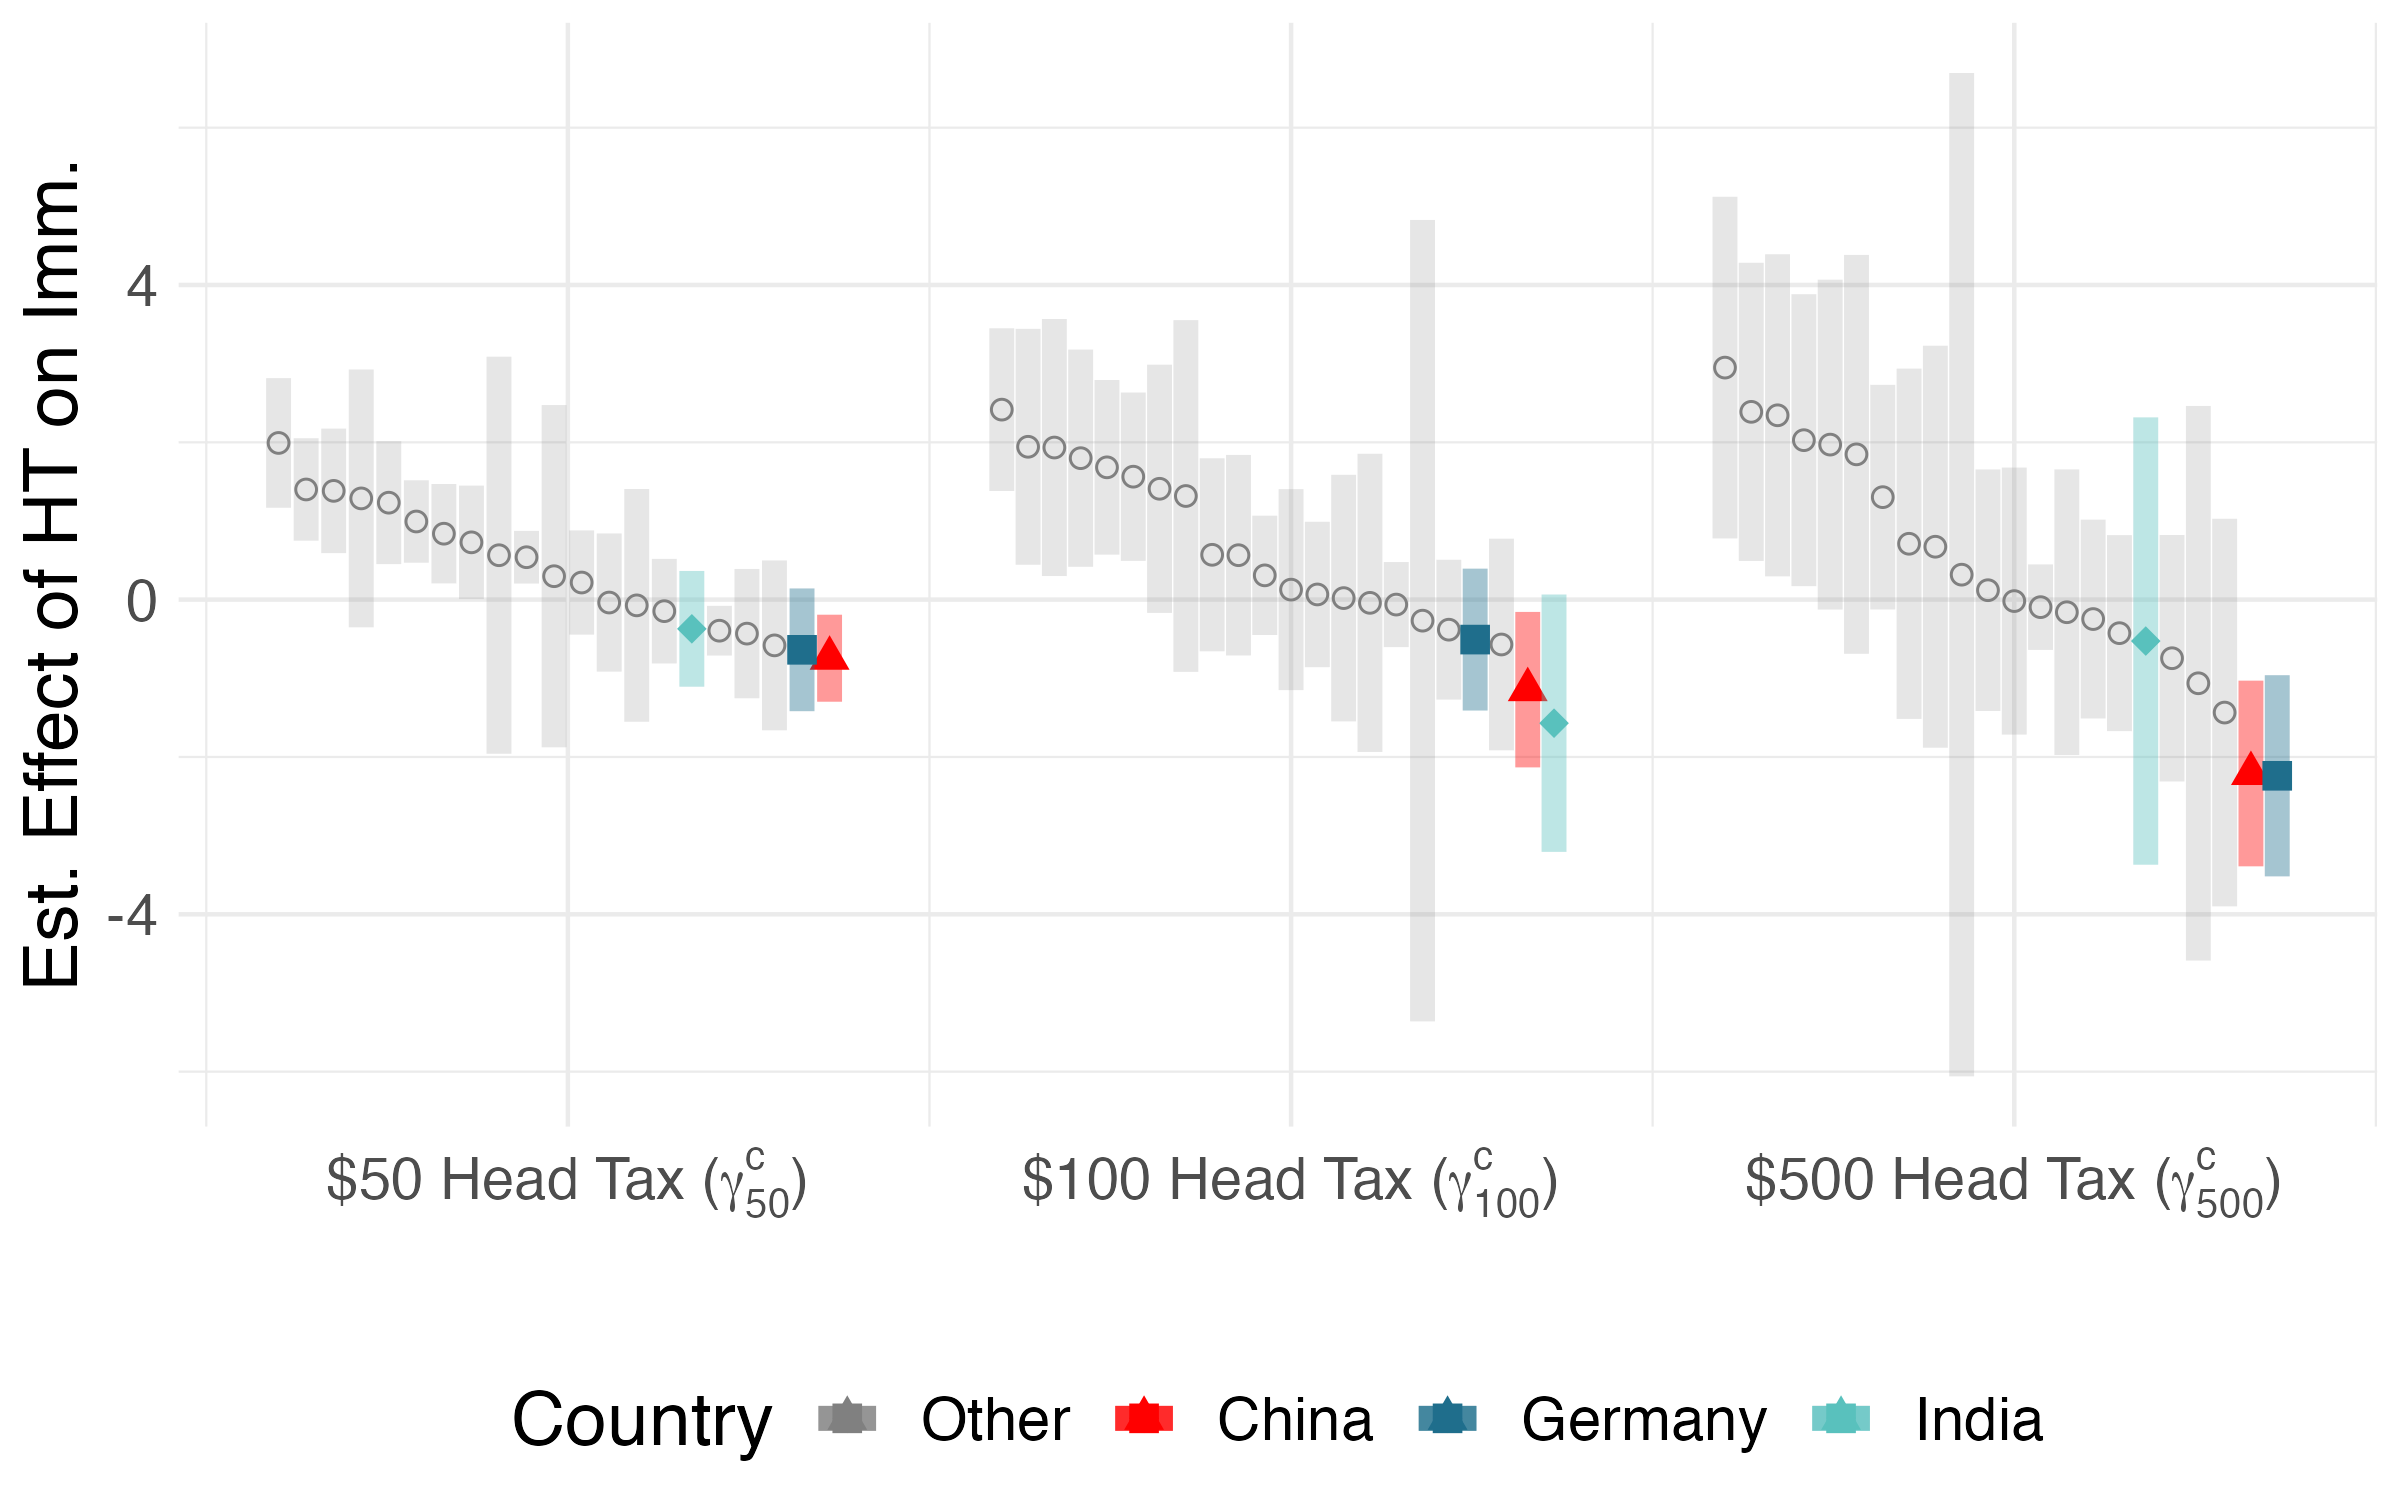
\includegraphics[width = 0.8\textwidth]{../../figs/slides/immflow_countries.png}
    \end{figure}
\end{frame}

\begin{frame}
    \label{theory1}
    \frametitle{Selection: Theoretical Framework Model Details \hyperlink{theory_main}{\beamerreturnbutton{Return}}}
    \textbf{Roy-Borjas:} \vspace{1mm}

    Model wage $w_c$ in country $c$ for worker with skill $s$ as: 
    \begin{equation}
        \ln(w_c) = \mu_c + \delta_c s 
    \end{equation}
    where $\mu_c$ represents baseline wage and $\delta_c$ represents return to skill.
    \vspace{1mm}

    Condition for migration with cost $\pi$:
    \begin{equation}
        \mu_1 + \delta_1 s - \pi > \mu_0 - \delta_0s
    \end{equation}
    where 1 indexes Canada, 0 indexes China.
    \vspace{1mm}
    \begin{itemize}
        \item $\delta_0 > \delta_1 \implies$ migration only occurs for $s < s^*$: negative selection
        \vspace{1mm}
        \item Increase in cost $\pi \implies $ decrease in $s^*$: \textbf{more negative selection}
    \end{itemize}
\end{frame}

\begin{frame}
    \label{theory2}
    \frametitle{Selection: Theoretical Framework Model Details 2 \hyperlink{theory_main}{\beamerreturnbutton{Return}}}
    \begin{figure}
        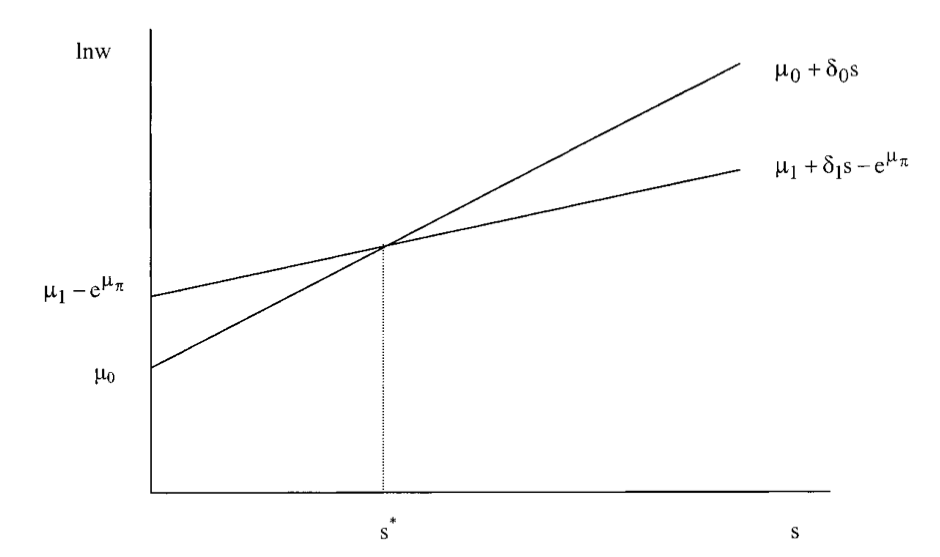
\includegraphics[width = 0.7\textwidth]{../../figs/slides/royborjas.png}
        \caption{\textcolor{gray}{Chiquiar and Hanson 2005 Fig 1}}
    \end{figure}
\end{frame}

\begin{frame}
    \label{theory3}
    \frametitle{Selection: Theoretical Framework Model Details 3 \hyperlink{theory_main}{\beamerreturnbutton{Return}}}
    \textbf{Chiquiar-Hanson:} \vspace{1mm}

    Now model cost as decreasing in skill: 
    \begin{equation}
        \ln(\pi) = \mu_{\pi} - \delta_{\pi}s 
    \end{equation} 
    \vspace{1mm}

    Condition for migration:
    \begin{equation}
        \mu_1 + \delta_1 s - \exp(\mu_{\pi} - \delta_{\pi}) > \mu_0 - \delta_0s
    \end{equation}
    \vspace{1mm}
    \begin{itemize}
        \item $\mu_{\pi}$ suff. large $\implies$ cost too high for lowest-skilled: intermediate selection \vspace{1mm}
        \item Increase in baseline cost $\mu_{\pi}$ and $\delta_{\pi}$: (likely) \textbf{more positive selection}
    \end{itemize}
\end{frame}

\begin{frame}
    \label{theory4}
    \frametitle{Selection: Theoretical Framework Model Details 4 \hyperlink{theory_main}{\beamerreturnbutton{Return}}}
    \begin{figure}
        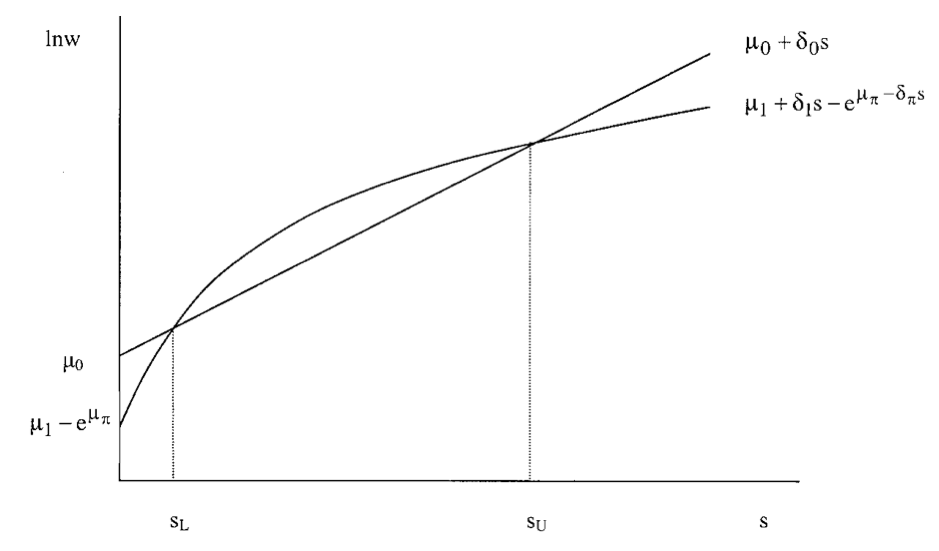
\includegraphics[width = 0.7\textwidth]{../../figs/slides/chiquiarhanson.png}
        \caption{\textcolor{gray}{Chiquiar and Hanson 2005 Fig 2}}
    \end{figure}
\end{frame}

\begin{frame}
    \label{baten_graph}
    \frametitle{Height of Various Chinese Populations \textcolor{gray}{Baten et al. 2010} \hyperlink{height2}{\beamerreturnbutton{Return}}}
    \centering
    \begin{figure}
        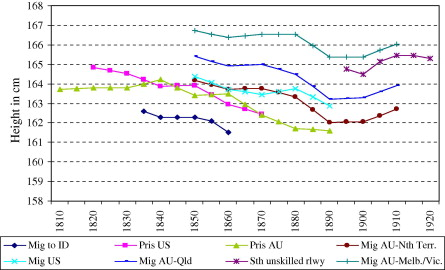
\includegraphics[width = 0.8\textwidth]{../../figs/slides/batenetal_heights.jpeg}
    \end{figure}
\end{frame}


\begin{frame}
    \label{reg_sel2}
    \frametitle{Results more mixed for Chinese vs. Japanese imm. \hyperlink{reg_sel1}{\beamerreturnbutton{Return}}}
    \centering
    \begin{table}
        \resizebox{0.9\textwidth}{!}{
% Table created by stargazer v.5.2.3 by Marek Hlavac, Social Policy Institute. E-mail: marek.hlavac at gmail.com
% Date and time: Tue, Jan 16, 2024 - 18:31:33
\begin{tabular}{@{\extracolsep{5pt}}lccc} 
\\[-1.8ex]\\[-1.8ex] & $\mathbb{P}[\text{Laborer}]$ & $\mathbb{P}[\text{Literate}]$ & $\mathbb{P}[\text{Owns House}]$ \\ 
\hline \\[-1.8ex] 
 $\hat{\beta}_{1}$ (Born in China) & 0.056$^{*}$ (0.031) & 0.023 (0.035) & $-$0.131$^{***}$ (0.025) \\ 
  $\hat{\gamma}_{100}^{DD}$ ($C_i \times$ \$100 Tax) & 0.050 (0.075) & 0.080 (0.079) & $-$0.007 (0.060) \\ 
  $\hat{\gamma}_{500}^{DD}$ ($C_i \times$ \$500 Tax) & $-$0.117$^{**}$ (0.052) & $-$0.114$^{**}$ (0.055) & 0.014 (0.042) \\ 
 \hline \\[-1.8ex] 
Dep. Var. Mean (Chinese) & 0.3582 & 0.6715 & 0.1325 \\ 
Observations & 2,190 & 1,864 & 2,190 \\ 
Adjusted R$^{2}$ & 0.017 & 0.008 & 0.060 \\ 
\end{tabular} 
}
    \end{table}
\end{frame}
\end{document}